\documentclass[12pt]{article}
\usepackage[utf8]{inputenc}
\usepackage[english]{babel}
\usepackage[a4paper,margin=1.2in,footskip=0.25in]{geometry}
\usepackage[dvipsnames]{xcolor}
\usepackage{amsthm}
\usepackage{amsmath}
\usepackage{amssymb}
\usepackage{mathtools}
\usepackage{bbm}
\usepackage{enumerate}
\usepackage{mathrsfs}
\usepackage{float}
\usepackage{chngcntr}
\usepackage{sectsty}
\usepackage{yfonts}
\usepackage{url}
\usepackage{wrapfig}
\usepackage{xfrac}
\usepackage{stmaryrd}
\usepackage{hyperref} % Uncommment to make references clickable
\usepackage{tikz}
\usepackage{minted} % For including Python code
\usepackage{tabularx}
\usepackage{setspace}
% This sets the line spacing
\setstretch{1}
% This sets the paragraph indent
\setlength{\parindent}{0cm}

% \definecolor{nice_blue}{RGB}{0,51,102}
% \definecolor{nice_blue}{RGB}{73, 115, 171}
\definecolor{niceBlue}{RGB}{48, 99, 165}
% \definecolor{nice_blue}{RGB}{61, 89, 171}
% \definecolor{nice_blue}{RGB}{65, 105, 225}
\definecolor{oxfordBlue}{RGB}{0, 33, 71}

% Configuring style of references
\hypersetup{
    colorlinks = True,
    allcolors = blue
}

% Makes equation numbering based on section
\counterwithin{equation}{section}

% Changing the styling of section and subsection titles. Comment to get default styling
\sectionfont{\centering\sffamily\scshape\color{black}}
\subsectionfont{\sffamily\color{black}}
\subsubsectionfont{\sffamily\color{black}}

%%%%%%%%%%%%%%%%%%%%%%%%%%% Defining environments %%%%%%%%%%%%%%%%%%%%%%%%%%%%%%%%%%%%%%%%
\newtheoremstyle{slimDefinitionStyle} % name
    {\topsep}                    	  % Space above
    {\topsep}                    	  % Space below
    {}			                   	  % Body font
    {}                           	  % Indent amount
    {\mdseries\scshape}			  	  % Theorem head font
    { ---}                         	  % Punctuation after theorem head
    {.5em}                       	  % Space after theorem head
    {}  % Theorem head spec (can be left empty, meaning ‘normal’)
\newtheoremstyle{slimTheoremStyle} 	% name
    {\topsep}                    	% Space above
    {\topsep}                    	% Space below
    {\itshape}                   	% Body font
    {}                           	% Indent amount
    {\mdseries\scshape}			 	% Theorem head font
    { ---}                         	% Punctuation after theorem head
    {.5em}                       	% Space after theorem head
    {}  % Theorem head spec (can be left empty, meaning ‘normal’)
\theoremstyle{slimTheoremStyle} % Comment this to get boldface theorem headers

\newtheorem{theorem}{Theorem}[section]
\newtheorem{proposition}{Proposition}[section]
\newtheorem{corollary}{Corollary}[theorem]
\newtheorem{lemma}[theorem]{Lemma}

% \theoremstyle{definition}
\theoremstyle{slimDefinitionStyle}
\newtheorem{definition}{Definition}[section]

\theoremstyle{remark}
\newtheorem{remark}{Remark}[section]
\newtheorem{assumption}{Assumption}
\newtheorem*{construction}{Construction}


%%%%%%%%%%%%%%%%%%%%%%%%%% Defining custom commands %%%%%%%%%%%%%%%%%%%%%%%%%%%%%%%%%%%%%%%
% Common fonts
\renewcommand{\cal}[1]{\mathcal{#1}}
\newcommand{\bb}[1]{\mathbb{#1}}
\renewcommand{\frak}[1]{\textfrak{#1}}
\newcommand{\scr}[1]{\mathscr{#1}}


% Common sets
\newcommand{\R}{\mathbb{R}}
\newcommand{\N}{\mathbb{N}}
\newcommand{\Z}{\mathbb{Z}}
\newcommand{\Q}{\mathbb{Q}}

% Expectation
\newcommand{\E}{\mathbb{E}}
\newcommand{\Ex}[1]{\mathbb{E}\left[ #1 \right]}
\newcommand{\ExCond}[2]{\mathbb{E} \left[\left. #1 \right| #2 \right]}

% Probability
\renewcommand{\P}{\mathbb{P}}
\renewcommand{\Pr}[1]{\mathbb{P} \left( #1 \right)}
\newcommand{\PrCond}[2]{\mathbb{P} \left( \left. #1 \right| #2 \right)}
\newcommand{\Ind}{\mathbbm{1}}

% Common distributions 
\newcommand{\dNorm}[2]{\mathcal(N)\left( #1, #2 \right)}
\newcommand{\dExp}[1]{\text{Exp} \left( #1 \right)}
\newcommand{\dBer}[1]{\text{Ber} \left( #1 \right)}
\newcommand{\dPo}[1]{\text{Poisson} \left( #1 \right)}
\newcommand{\dBin}[2]{\text{Binomial} \left( #1, #2 \right)}


% Miscellaneous math stuff
\newcommand{\defeq}{\vcentcolon=}
\newcommand{\eqdef}{=\vcentcolon}
\DeclarePairedDelimiter\ceil{\lceil}{\rceil}
\DeclarePairedDelimiter\floor{\lfloor}{\rfloor}
\DeclarePairedDelimiter\bbracket{\llbracket}{\rrbracket}
\DeclarePairedDelimiterX{\norm}[1]{\lVert}{\rVert}{#1}

\newcommand*\circled[1]{\tikz[baseline=(char.base)]{
            \node[shape=circle,draw,inner sep=2pt] (char) {#1};}}



\usepackage{fancyheadings}
\pagestyle{fancy}
\rhead{Candidate number --- 1006416}

\begin{document}

\begin{titlepage}
   \begin{center}
       \vspace*{1cm}
 
       \textbf{{\huge Branching Random Walks \\ with Selection}}
       \vspace{1.5cm} \\
       \textbf{Candidate number: 1006416}
       \vspace{0.5cm} \\
       Supervised by Prof. Julien Berestycki 
       \vspace{0.5cm} \\
       Dissertation on a topic in Statistics \linebreak presented for MMath in Mathematics and Statistics
       \vspace{0.3cm} \\
       Trinity term 2019
       \vfill
 
       
\includegraphics[width=0.5\textwidth]{graphics/oxford_logo.png}
 
 
   \end{center}
\end{titlepage}

\tableofcontents
\newpage

\section*{Notation}
\begin{tabularx}{\linewidth}{ l X }
$\N$ 						& $\{0, 1, 2, ...\}$ \\
$\R$ 						& The set of real numbers \\
$[n]$ 					& $\{ 1, 2, ..., n\}$  \\
$\bbracket{n, m}$ 		& $\{n, n+1, ..., m\}$ \\
$a \land b$				& $\min\{ a, b\}$ \\
$a \lor b$				& $\max\{ a, b\}$ \\
$f(x) \sim g(x),\,\text{as }x\to x_0$   & $\lim\limits_{x \to x_0} \frac{f(x)}{g(x)} = 1$ \\
$f(x) = o(g(x)),\,\text{as }x\to x_0$   & $\lim\limits_{x \to x_0} \frac{f(x)}{g(x)} = 0$ \\
$f(x) = \cal{O}(g(x))$ & $\exists\,M, R > 0\text{ such that } |f(x)| \leq M g(x)\text{ for all } x > R$ \\
$f(x) = \Theta(g(x))$ & $\exists\,M_1, M_2, R > 0\text{ such that } M_1 g(x) \leq f(x) \leq M_2 g(x)\text{ for all } x > R$ \\
$f(x) \propto g(x)$	& $\exists\,\alpha > 0$ such that $f(x) = \alpha g(x)$ for all $x$ \\
$A^\circ$ & Interior of $A \subseteq \R$ \\
$\operatorname*{dom}f$ & Domain of $f$, the set of values on which $f$ is defined \\
$\P$ & Underlying probability measure \\
$\E[\cdot], \bb{V}(\cdot)$ & Expectation and variance with respect to $\P$ \\
$L^p,\,p\geq 1$     		& Lebesgue space of random variables with finite $p$'th moment \\
$\operatorname*{ess\,sup}f$ & $||f||_{L^\infty}\defeq\inf\{ M > 0\,:\, |f|\leq M\text{ almost everywhere}\}$ \\
$C^k, C^\infty$				& Space of functions with continuous $k$'th derivative and space of smooth functions respectively \\
BRW						& Branching random walk \\
N-BRW					& Branching random walk with selection \\
$(\bb{T}, V)$			& Representation of a BRW with genealogical tree $\bb{T}$ and particle positions $(V(x))_{x \in \bb{T}}$ \\
$(X_n)_{n \geq 0}$ 		& Used to denote the $N$-BRW in question throughout the essay \\
$\scr{L}$				& Point process driving $(X_n)_{n \geq 0}$ \\
$\min \scr{L},\,\max \scr{L}$			& Position of right- and leftmost particle in the point process $\scr{L}$, provided they exist \\
$\scr{L}(k)$ 			& Position of $k$'th particle from the right given it exists, otherwise equal to $\min \scr{L}$ \\
$X$ 					& The distribution of the spine of $(X_n)_{n \geq 0}$ \\
$\psi$ 					& Logarithmic moment generating function of $\scr{L}$ \\
$\frak{M}$				& A specific subset of the counting measures on $\R$ (see Section \ref{sec:BRW_THEORY})\\
$\frak{M}_n$			& Measures in $\frak{M}$ with total mass $n$ \\
$\ceil{\cdot},\,\floor{\cdot}$ & Ceiling and floor functions respectively 
\end{tabularx}\hfill
\newpage
\input{Introduction}
\section{BRANCHING RANDOM WALKS}\label{sec:BRW_THEORY}

In this section we present some important results for BRWs that satisfy an exponential moment assumption. At the heart of the result is a probability change which enables us to say things about the BRW via its spine, a one-dimensional random walk. The idea was first introduced for BRWs by Lyons in \cite{lyons1997simple}. In our exposition we rely on \cite{mallein2018n} and \cite[Section 4.7]{shi2015branching}. 

\subsection{Definition and notation}
It will be convenient to think of BRWs and $N$-BRWs as stochastic processes taking values in the set $\frak{M}$ of counting measures $\mu$ on $\R$ which put non-negative integer mass on every real number and further satisfy $0 < \mu([x, \infty)) < \infty$ for some $x \in \R$. The latter condition is needed for the phrase `rightmost particles' to be meaningful. We will write $\frak{M}_N \subset \frak{M}$ for measures which have total mass $N$ and $\delta_{x_0} \in \frak{M}_1$ for the unit mass at $x_0$. The interpretation is that if $\mu$ is the value of the ($N$-)BRW at some time $n$, then there are exactly $\mu(\{x\})$ particles at position $x$ at time $n$. There is a natural partial order on $\frak{M}$: we say that $\mu \preceq \nu$ if $\mu([x, \infty)) \leq \nu([x, \infty))$ for all $x \in \R$. \\

% For $\mu \in \frak{M}$ and scalars $\alpha, \beta \in \R$ we will write
% \begin{equation}\nonumber
% \alpha \mu + \beta \defeq \sum\limits_{x \in \R} \mu(\{x\}) \delta_{\alpha x + \beta}. 
% \end{equation} 

For random elements (also referred to as point processes) $\scr{L}, \scr{G}$ of $\frak{M}$ we say that $\scr{L} \preceq \scr{G}$ if there exists a coupling $(\scr{L}, \scr{G})$ such that $\scr{L} \preceq \scr{G}$ almost surely. In summations involving $\scr{L}$ we'll write $\sum_{l \in \scr{L}} [\cdots]$ for the sum over positions $l$ of the particles in $\scr{L}$ and $\#\scr{L}$ for the total mass of $\scr{L}$. We'll further write $\scr{L}(k)$ for the random variable defined as follows: if $\scr{L}$ has at least $k$ particles then set $\scr{L}(k)$ to be the position of the $k$-th particle from the right; otherwise set it equal to $\min \scr{L}$. We will always assume 
\begin{equation}\label{eqn:TreeAssumptions}
1 \leq \# \scr{L} \qquad \text{almost surely} \qquad\text{and}\qquad 1 < \Ex{\# \scr{L}}. 
\end{equation}
The former is necessary and sufficient for the $N$-BRW to survive with positive probability, while the latter ensures that we avoid the trivial case of $\# \scr{L} \equiv 1$ where the model reduces to $N$ independent random walks. \\

\begin{definition}[$N$-BRW]\label{def:NBRW}
We call an $\frak{M}$-valued Markov chain $(X_n)_{n \geq 0}$ an $N$-BRW driven by the point process $\scr{L}$ if $X_0 \in \frak{M}_N$ is deterministic and given $X_n$, $X_{n+1}$ is defined as follows. Each particle in $X_n$ gives birth to children according to i.i.d. copies of $\scr{L}$ centred around the parent. Then, out of all children the $N$ rightmost are chosen to form the next generation. 
\end{definition}

Not surprisingly, regular BRWs are defined similarly except no selection happens. Alternatively one can take $N = \infty$ in Definition \ref{def:NBRW} to get the definition of BRWs. In more mathematical terms we can construct ($N$-)BRWs using the notation we have introduced so far: Suppose that $\scr{L}$ is the point process driving the ($N$-)branching random walk $(X_n)_{n\geq0}$ which is given up to time $n\geq0$. Define 
\begin{equation}\label{eqn:GeneralConstruction}
\widetilde{X}_{n+1} \defeq \sum\limits^{\# X_n}_{j=1} \sum\limits_{l \in \scr{L}_{n, j}} \delta_{X_n(j) +  l}. 
\end{equation}
If $X$ is a regular BRW just set $X_{n+1} \defeq \widetilde{X}_{n+1}$, in the $N$-BRW case set $X_{n+1}$ to be the $N$ rightmost particles of $\widetilde{X}_{n+1}$. This construction gives way to a natural and important coupling between ($N$-)BRWs. It was first described in \cite{exp_tails}, and the way we present it here is more general and similar to \cite{mallein2018n} Lemma 4.1:

\begin{lemma}\label{lem:monotonicity}
Let $1 \leq N_1 \leq N_2$ be fixed and $\mu_i \in \frak{M}_{N_i}$ for $i=1,2$ with $\mu_1 \preceq \mu_2$. Take two random elements $(\scr{L}_i)_{i =1,2} \in \frak{M}$ satisfying $\scr{L}_1 \preceq \scr{L}_2$. If $\{(X^{(i)}_n)_{n\geq0}\}_{i=1,2}$ are two ($N_i$-)BRWs driven by the point processes $(\scr{L}_i)_{i = 1,2}$ and are started from $(\mu_i)_{i = 1,2}$ respectively, then there exists a coupling such that $X^{(1)}_n \preceq X^{(2)}_n$ almost surely for all $n \geq 0$. 
\end{lemma}

\begin{proof}[Sketch of proof]
We construct the coupling inductively. The base case clearly holds so suppose that we are given $X^{(1)}_n \preceq X^{(2)}_n$ up to some $n \geq 0$. Independently take $N_2$ i.i.d. copies $\{(\scr{L}^{(1)}_i, \scr{L}^{(2)}_i)\}^{N_2}_{i=1}$ of the coupling of $\scr{L}_1$ and $\scr{L}_2$ under which $\scr{L}_1 \preceq \scr{L}_2$ almost surely. Using these, construct $\widetilde{X}^{(1)}_{n+1}$ and $\widetilde{X}^{(2)}_{n+1}$ as in (\ref{eqn:GeneralConstruction}). If the $X^{(i)}$ are regular BRWs just set $X^{(i)}_{n+1} = \widetilde{X}^{(i)}_{n+1}$, if they are $N_i$-BRWs take the rightmost $N_i$-particles. Either way, we have $X^{(1)}_{n+1} \preceq X^{(2)}_{n+1}$ as desired. 
\end{proof}	


Let us introduce more notation that's commonly used in the literature of BRWs. For a BRW started from a single particle at zero, denote by $\bb{T}$ the genealogical tree of the system and write $(V(x))_{x \in \bb{T}}$ for the positions of the particles on the real line. Further let $|x|$ be the generation of $x$ and write $x_i$ for the ancestor of $x$ in generation $i$ so that $x_0 = \varnothing$ where $\varnothing$ denotes the root of $\bb{T}$. Let $(\bb{T}, V)$ be a BRW started from $0$ and $\scr{L} \in \frak{M}$ be the point process that governs its evolution. It is easy to see then that $\bb{T}$ is a Galton-Watson tree with $\# \scr{L}$ as its reproduction law. 

\subsection{The Many-to-One Lemma}

Suppose now that $V$ satisfies
\begin{equation}\label{eqn:BRW_V_Ass}
\E \sum\limits_{|x|=1} e^{V(x)} = 1. 
\end{equation}
Then we can define a random variable $X$ by giving it's distribution function: 
\begin{equation}\nonumber
\Pr{X \leq u} = \E \sum\limits_{|x| = 1} \Ind_{\{V(x) \leq u\}} e^{V(x)}. 
\end{equation}
If $(S_n)_{n\geq0}$ is a random walk with step distribution $X$ started from $S_0 = 0$ then we have the following result:
\begin{lemma}[Many-to-one]\label{lem:many_to_one}
Let $(\bb{T}, V)$ be a BRW governed by the point process $\scr{L}$ which satisfies (\ref{eqn:BRW_V_Ass}). Take $n \geq 1$ and let $g:\R^n \to \R$ be measurable. Provided the integrals exist, 
\begin{equation}\nonumber
\E \sum\limits_{|x| = n} g(V(x_1), ...,V(x_n)) = \Ex{e^{-S_n} g(S_1, ...,S_n)}. 
\end{equation}
\end{lemma}
\begin{remark}
One might ask themselves what use the Many-to-One lemma is if it relies on assumption (\ref{eqn:BRW_V_Ass}). However, for a large class of point processes there is a simple transformation that puts them in the desired form as will se in Section \ref{subsec:centering_the_spine}. 
\end{remark}

Lemma \ref{lem:many_to_one} is a consequence of the Spinal Decomposition Theorem, one of the most important tools in the study of BRWs. For more details we refer the reader to Chapter 4 of \cite{shi2015branching} and Section 4.7 in particular. $(S_n)_{n\geq0}$ is sometimes called the random walk associated with the BRW $(\bb{T}, V)$. An application of the many-to-one formula with $n=1$ and $g(x) = x e^x$ yields $\E X = \E \sum_{|x|=1} V(x) \exp(V(x))$ while for the variance we get $\bb{V}(X) = \E \sum_{|x|=1} V(x)^2 \exp(V(x)) - (\E X)^2$ provided that the necessary integrability conditions hold. \\





\subsection{Logarithmic moment generating functions}\label{subsec:moment_generating_functions}
Suppose that $(\bb{T}, V)$ is a BRW with point process $\scr{L}$ and define the associated logarithmic moment generating function to be
\begin{equation}\nonumber
\psi(t) \defeq \log \E \int_\R e^{t x} \scr{L}(dx) = \log \E \sum\limits_{x \in \bb{T}: |x|=1} e^{t V(x)} 
\end{equation}
for $t \in \R$ where it is defined. A standard assumption in the BRW literature is the following: 
\begin{equation}\label{eqn:BRW_generator_finite}
0 < \sup\operatorname*{dom} \psi = \sup\{ t > 0 \mid\, \psi(t) < \infty \}. 
\end{equation}
This assumption controls the right tail of the point process $\scr{L}$ and ensures that the rightmost particle has an asymptotic velocity by Theorem 1.3 \cite{shi2015branching}. In Section \ref{sec:poly} we will briefly review some results that don't rely on this assumption. Let $t_1 \neq t_2 \in \operatorname*{dom} \psi$ and $\lambda \in (0, 1)$. Since $x \to e^x$ is convex we have
\begin{align*}
\exp [\psi(\lambda t_1 + (1 - \lambda) t_2)] &= \E \sum\limits_{|x| = 1} e^{\lambda (t_1 V(x))+ (1 - \lambda) (t_2 V(x))} \\
									  &\leq	\lambda e^{\psi(t_1)} + (1 - \lambda)e^{\psi(t_2)} < \infty. 
\end{align*} 
This shows that the domain of $\psi$ is an interval and that the function $\Psi \defeq \exp(\psi)$ is convex. Suppose now that $\scr{L}$ satisfies (\ref{eqn:BRW_V_Ass}) so that $\Psi(1) = 1$. Then by the Many-to-One lemma for all $t \in \operatorname*{dom} \psi$ we have
\begin{equation}
\Psi(t) = \Ex{e^{(t - 1)X}}. 
\end{equation}
By standard results on moment generating functions we know that $t \mapsto \Ex{e^{(t - 1)X}}$ is $C^\infty$ on $(\operatorname*{dom} \psi)^\circ$ moreover
its derivatives are given by 
\begin{equation}
\frac{d^n}{dt^n} \Psi(t) = \Ex{X^n e^{(t - 1)X}} = \E \sum\limits_{|x| = 1} V(x)^n e^{t V(x)}. 
\end{equation}
Furthermore, if $[a, b] \subset \operatorname*{dom} \psi$ then left and right derivatives of all orders exist satisfying $\Psi^{(n)}_+(a) = \Ex{X^n e^{(a - 1)X}}$ and $\Psi^{(n)}_-(b) = \Ex{X^n e^{(b - 1)X}}$ where $X^n e^{(a - 1)X}$ and $X^n e^{(b - 1)X}$ are quasi-integrable. As $\Psi$ is convex we also know that ${\Ex{X^n e^{(a - 1)X}} < \infty}$ and that $\Ex{X^n e^{(b - 1)X}} > -\infty$. 





\subsection{Centering the spine}\label{subsec:centering_the_spine}
Shi \cite{gantert2008asymptotics} notes that the condition $\psi'(1) = 0 = \psi(1)$ is `fundamental to various universality behaviours of BRWs'. This condition ensures that the rightmost particle in the corresponding BRW (wrihout selection) has asymptotic velocity equal to $0$. However, for general $\psi$ it is not necessarily the case that $1 \in \operatorname*{dom}\psi$. Even if $\psi(1) < \infty$, if $1$ is the right endpoint of $\operatorname*{dom}\psi$ then the (right-)derivative might be infinite. We now discuss when this assumption can be made. \\

For scalars $\alpha > 0, \beta \in \R$ let $\gamma_{\alpha, \beta} : \scr{P}(\R) \to \scr{P}(\R)$ be the map on the powerset of $\R$ given by
\begin{equation}
\gamma_{\alpha, \beta}(A) = \{x \in \R\,:\, (x - \beta) / \alpha \in A\}
\end{equation}
for each $A \subseteq \R$. Putting it more simply, $\gamma_{\alpha, \beta}$ maps a subset $A \subseteq \R$ to the set obtained by shrinking $A$ by $\alpha$ and translating it to the left by $\beta$. Take a BRW $(\bb{\widehat{T}}, \widehat{V})$ with point process $\widehat{\scr{L}}$ and logarithmic moment generating function $\widehat{\psi}$. For some $0 < t^* \in \operatorname*{dom} \psi$, define
\begin{equation}\label{eqn:transformation}
\scr{L} \defeq \widehat{\scr{L}} \circ \gamma_{t^* , - \widehat{\psi}(t^*)}. 
\end{equation}
Clearly $\scr{L}$ is a point process much like $\widehat{\scr{L}}$ so we can consider $(\bb{T}, V)$, the corresponding BRW. It is easy to see that $V$ and its logarithmic moment generator function $\psi$ are given by 
\begin{equation}\label{eqn:transformation2}
V(x) = t^* \widehat{V}(x) - |x| \widehat{\psi}(t^*) \qquad\text{and}\qquad \psi(t) = \widehat{\psi}(t t^*) -t \widehat{\psi}(t^*) 
\end{equation}
for $x \in \bb{T}$. The form of (\ref{eqn:transformation}) is chosen precisely so that $\psi(1) = 0$. Differentiating, we obtain
\begin{equation}
\psi'(t) = t^* \widehat{\psi}'(t t^*) - \widehat{\psi} (t^*). 
\end{equation}
We can achieve $\psi'(1) = 1$ if and only if there exists $t^*$ such that $t^* \widehat{\psi}'(t^*) = \widehat{\psi} (t^*)$. For simplicity we will also require $t^*$ be in the interior of the domain, in summary:
\begin{equation}\label{eqn:t*exists}
\exists\,t^* \in (0, \infty) \cap (\operatorname*{dom}\widehat{\psi})^\circ\text{ such that } t^* \widehat{\psi}'(t^*) = \widehat{\psi} (t^*). 
\end{equation}
Since $t^*$ is chosen to be in the interior of $\operatorname*{dom}\widehat{\psi}$, it follows that $\psi$ is smooth in a neighbourhood of $1$. In particular
\begin{equation}\nonumber
\E{X} = \psi'(1) = 0 \qquad\text{and}\qquad \bb{V}(X) = \psi''(1) = (t^*)^2 \widehat{\psi}''(t^*) < \infty. 
\end{equation} 
\begin{remark}
Note that if we didn't insist that $t^*$ be in the interior of $\operatorname*{dom} \widehat{\psi}$ then it would be possible for $t^*$ to be the right endpoint of the domain. In this case we might have $\E X = t^* \widehat{\psi}'_-(t^*) - \widehat{\psi}(t^*)$ but $\widehat{\psi}''_-(t^*) = \bb{V}(X) = \infty$. This is briefly explored in Section \ref{subsec:alpha_stable_spine}. 
\end{remark}
Let $x_{max} = \operatorname*{ess\,sup} \{\max\widehat{\scr{L}}\}$ be the essential supremum of the rightmost particle in a realisation of $\widehat{\scr{L}}$. Jaffuel gives the following characterization of when $t^*$ exists:
\begin{proposition}[{{\cite[Proposition A.2]{jaffuel2227critical}}}]\label{prop:jaffuel}
Suppose $[0, \infty) \subset \operatorname*{dom}\widehat{\psi}$. Then there exists $t^* > 0$ such that (\ref{eqn:t*exists}) holds if and only if 
\begin{equation}\nonumber
x_{max} = \infty \qquad \text{or} \qquad\E \sum_{l \in \widehat{\scr{L}}} \Ind_{\{ l = x_{max}\}} < 1. 
\end{equation}
\end{proposition}
In words, assuming $\Ex{\#\widehat{\scr{L}}} < \infty$ and $\widehat{\psi}(t) < \infty$ for all $t>0$, there exists $t^* > 0$ satisfying (\ref{eqn:t*exists}) if and only if (a) the particles in $\scr{L}$ can be arbitrarily far to the right or (b) if $\scr{L}$ doesn't put too much weight on $x_{max}$. For a complete discussion (including the case $\sup \operatorname*{dom} \widehat{\psi} < \infty$) see the appendix of \cite{jaffuel2227critical}.



%  Provided differentiability of $\psi$ and that the order of integration and differentiation can be interchanged - which is the case for sufficiently regular models - it follows then that $d^n \psi(t) / dt^n = \E \sum_{|x|=1} V^n(x) \exp(t V(x))$ and in particular 
% \begin{equation}\label{eqn:RWCentred}
% \E{X} = \psi'(1) = 0 \qquad\text{and}\qquad \bb{V}(X) = \psi''(1) = (t^*)^2 \widehat{\psi}''(t^*). 
% \end{equation}



\subsection{Killed below a linear boundary}

Let $(\bb{T}, V)$ be the BRW governed by $\scr{L}$ with logarithmic moment generating function $\psi$ which is obtained after the transformation (\ref{eqn:transformation}) with $t^*$ as in (\ref{eqn:t*exists}). We now state two results from \cite{gantert2008asymptotics} that we will use in Section \ref{sec:light_tails}. The assumptions necessary to apply them are as follows. Suppose 
\begin{equation}\label{ass:killed_assumption_Lp}
1 < \Ex{(\# \scr{L})^{1 + \delta}} < \infty\qquad\text{ for some } \delta > 0, 
\end{equation}
and that 
\begin{equation}\label{ass:DacyingTails}
0 \in (\operatorname*{dom} \psi)^\circ. 
\end{equation}

Let $1 \leq m \leq \infty$ and call a sequence of vertices $(u_n)_{0 \leq n \leq m}$ a path if $u_i$ is the parent of $u_{i+1}$ for each $0 \leq i \leq m-1$. For $v \in \R$ we say that the vertex $u \in \bb{T}$ is $(m, v)$-good if there exists a path $(u_n)_{0 \leq n \leq m}$ with $u_0 \defeq u$ such that $V(u_i) - V(u) \geq vi$ for all $i \in [m]$. This is essentially saying that there exists a path starting at $u$ that stays to the right of the space-time line through $(|u|, V(u))$ with slope $v$, for at least $m$ steps. Under assumptions (\ref{ass:killed_assumption_Lp}) and (\ref{ass:DacyingTails}) the following holds. 
\begin{theorem}[{{\cite[Theorem 1.2]{gantert2008asymptotics}}}]\label{thm:infty_good}
Let $\rho(\infty, - \epsilon)$ denote the probability that the root of $(\bb{T}, V)$ is $(\infty, - \epsilon)-good$. Then, as $\epsilon > 0$ goes to zero, 
\begin{equation}\nonumber
\log\rho(\infty, - \epsilon) = - \pi \sqrt{\frac{\bb{V}(X) + o(1)}{2 \epsilon}}. 
\end{equation}
\end{theorem}

A similar result can be obtained for the probability of observing a $(m, - \epsilon)$-good root with $m$ finite:
\begin{theorem}[{{\cite[Consequence of proof of Theorem 1.2]{gantert2008asymptotics}}}]\label{thm:finite_good}
Let $\rho(m, - \epsilon)$ denote the probability that the root of $(\bb{T}, V)$ is $(m, - \epsilon)$-good. For any $0 < \beta < \bb{V}(X)$, there exists $\theta > 0$ such that for all large $m$, 
\begin{equation}\nonumber
\log \rho(m, - \epsilon) \leq - \pi \sqrt{\frac{\bb{V}(X) - \beta}{2 \epsilon}}, \qquad \text{with } \epsilon \defeq \theta m^{-2/3}. 
\end{equation}
\end{theorem}

\newpage
\section{N-BRW WITH LIGHT TAILS}\label{sec:light_tails}

In \cite{exp_tails} Bérard and Gouéré studied the $N$-BRW whose point process is given by two independent draws from a distribution $p$ that has finite moment generating function in some neighbourhood of zero and whose spine can be centred (see \ref{eqn:t*exists}). In this section we adapt their results to the more general case of $N$-Branching Random Walks with finite logarithmic moment generating function in a neighbourhood of zero whose spine can be centered. Loosely speaking we extend their results to the case where the number of offspring are random and their position not necessarily independent of each other. We use the methods of \cite{exp_tails} for most proofs, adding details and adapting the arguments as necessary. 

\subsection{The model}\label{subsec:The_model}
Consider the BRW $(\widehat{\bb{T}}, \widehat{V})$ governed by the point process $\widehat{\scr{L}}$ with logarithmic moment generating function $\widehat{\psi}$. Assume that (\ref{eqn:TreeAssumptions}), (\ref{eqn:t*exists}) and (\ref{ass:DacyingTails}) holds. Let $(\widehat{X}_n)_{n \geq 0}$ be the corresponding $N$-BRW and write $\max \widehat{X}_n$ and $\min \widehat{X}_n$ for the position of the right- and leftmost particle of $\widehat{X}_n$. We will show that 
\begin{equation}\nonumber
\hat{v}_N \defeq \lim_{n \to \infty} n^{-1}\max\widehat{X}_n = \lim_{n \to \infty} n^{-1}\min\widehat{X}_n
\end{equation} 
exists in $L^1$ and almost surely. The main result in this section is the analogue of Theorem 1 of \cite{exp_tails}: 
\begin{theorem}\label{thm:ExpTails_BrunDer_non_transformed}
As $N$ goes to infinity, 
\begin{equation}\nonumber
\widehat{v}_N = \widehat{\psi}'(t^*) - \frac{\pi^2 t^* \widehat{\psi}''(t^*)}{2 (\log N)^2} + o((\log N)^{-2}). 
\end{equation}
\end{theorem}


% Notice that if instead of $\widehat{\scr{L}}$ we used the point process $\widehat{\scr{L}}_N$ defined as $\widehat{\scr{L}}_N \defeq \sum^{N \land \# \scr{L}}_{i=1} \delta_{\scr{L}(i)}$ the resulting $N$-BRW would be exactly the same. Since $\# \widehat{\scr{L}}_N \leq N$ almost surely we see that assumption (\ref{ass:killed_assumption_Lp}) can be taken for granted. 


It will be more convenient to work with the BRW that is obtained after the transformation (\ref{eqn:transformation}). The resulting BRW will be denoted by $(\bb{T}, V)$ with point process $\scr{L}$ and logarithmic moment generating function $\psi$ that satisfies (\ref{eqn:BRW_V_Ass}). Observe that the associated random walk $(S_n)_{n \geq 0}$ with step distribution $X$ then satisfies (\ref{eqn:RWCentred}), i.e. $\E X = 0$. Let $X \defeq (X_n)_{n \geq 0}$ denote the $N$-BRW with point process $\scr{L}$ and take $X_0 \in \frak{M}_N$ deterministic. Assuming they exists, $v_N \defeq \lim_{n \to \infty} n^{-1} \max X_n$ is related to $\hat{v}_N$ by 
\begin{equation}\label{eqn:speed_relation}
v_N + \widehat{\psi}(t^*)= \hat{v}_N t^*, 
\end{equation}
as can be seen from (\ref{eqn:transformation2}). Therefore, what we will prove the following:
\begin{theorem}[Brunet-Derrida behaviour, centred form] \label{thm:ExpTails_BrunDer}
As $N$ goes to infinity, 
\begin{equation}\nonumber
v_N = - \frac{\pi^2 (t^*)^2 \widehat{\psi}''(t^*)} {2 (\log N)^2} + o((\log N)^{-2}). 
\end{equation}
\end{theorem}

\subsection{Properties of the model}
Clearly for all $t\in\R$ and $k \geq 1$ we have 
\begin{equation}\nonumber
0 \leq e^{t\, \scr{L}_{n,j}(k)} \leq \sum_{|x|=1} e^{t\, V(x)}
\end{equation} so by assumption (\ref{ass:DacyingTails}) the $\scr{L}_{n,j}(k)$ have finite moment generating function in a neighbourhood of zero which implies exponentially decaying tails. It follows by Lemma \ref{lem:ExpTailsMax} that $\min X_n$ and $\max X_n$ are integrable and hence finite almost surely. Let $d(X_n) \defeq \max X_n - \min X_n$ be the diameter of $X_n$. The following result is analogous to Corollary 1 of \cite{exp_tails} and says that the diameter doesn't get too large:

\begin{proposition}\label{prop:diameter}
For any $N \geq 1$ and initial population $X_0 \in \frak{M}_N$, we have 
\begin{equation}\nonumber
\frac{d(X_n)}{n} \xrightarrow[n \to \infty]{a.s.,\, L^1} 0. 
\end{equation}
\end{proposition}

\begin{remark}
In \cite{mallein2018n} Mallein shows something stronger: he shows that there exists $C > 0$ such that for all $N$, 
\begin{equation}\nonumber
\Pr{d(X_n) > y} \leq C \left( \frac{N(\log N + \log y)}{y}\right)^2
\end{equation}
for all sufficiently large $n$. Using this we can get an upper bound on $\E\, d(X_n)$:
\begin{equation}\nonumber
\E\, d(X_n) = \int\limits_0^\infty \Pr{d(X_n) > x} dx \leq 1 + C N^3 \int\limits^\infty_N \left[\frac{\log x}{x}\right]^2 dx = 1 + C N^2[ \log^2 N + 2 \log N + 2]. 
\end{equation}
\end{remark}

\begin{figure}[!h]
\centering
\begin{minipage}{0.45\textwidth}
  \centering
  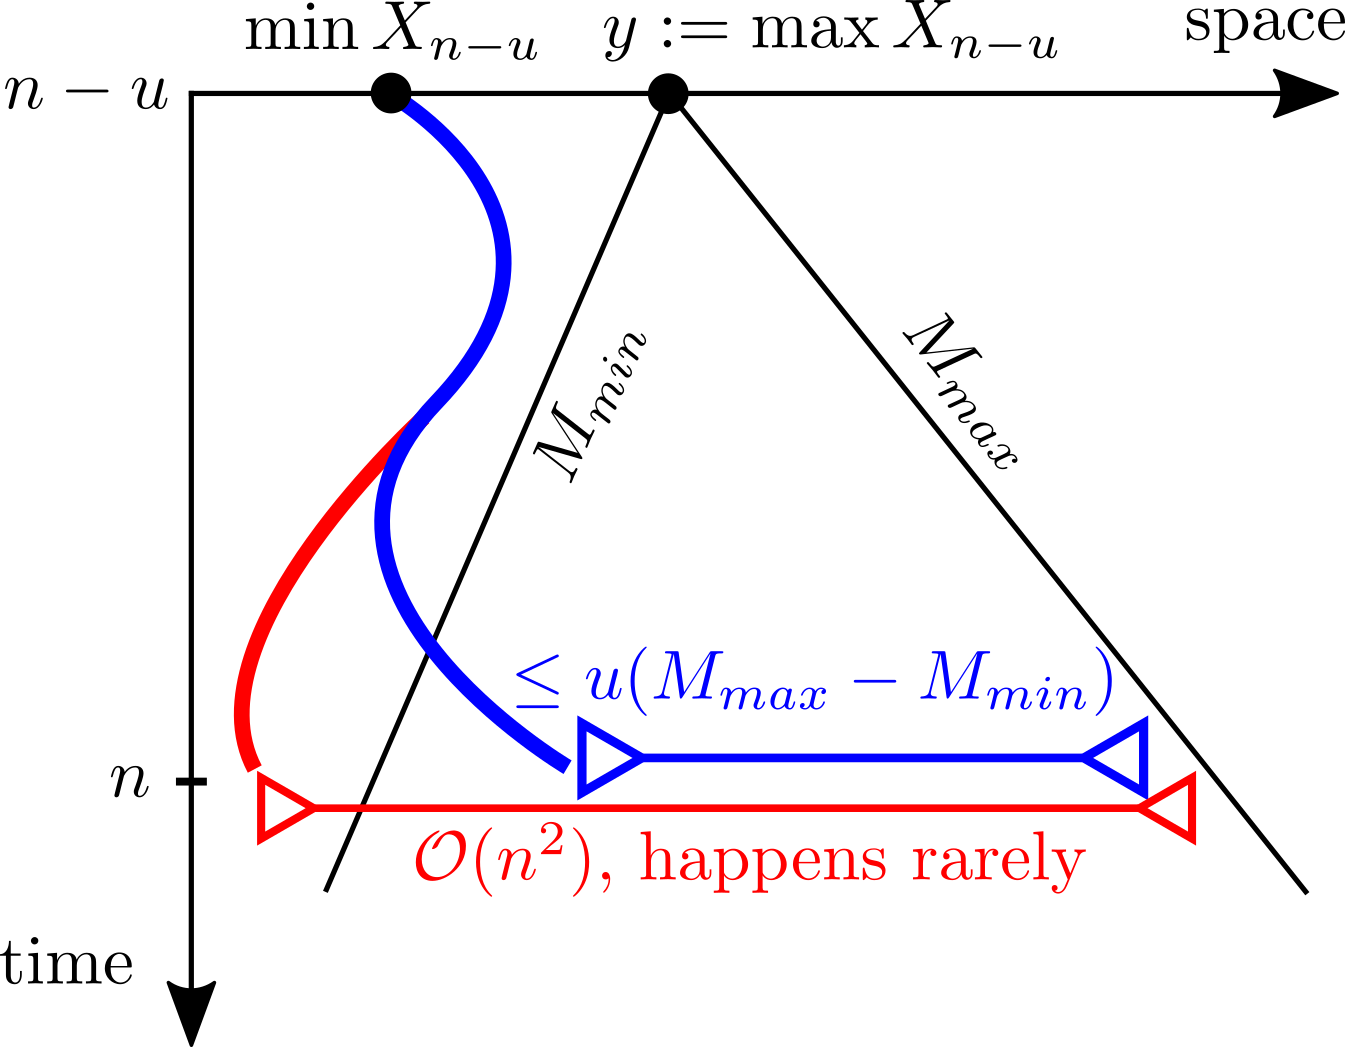
\includegraphics{graphics/g2}
  \caption{Proof of Proposition \ref{prop:diameter}. }
  \label{fig:diam_proof}
\end{minipage}\hfill%
\begin{minipage}{0.45\textwidth}
  \centering
  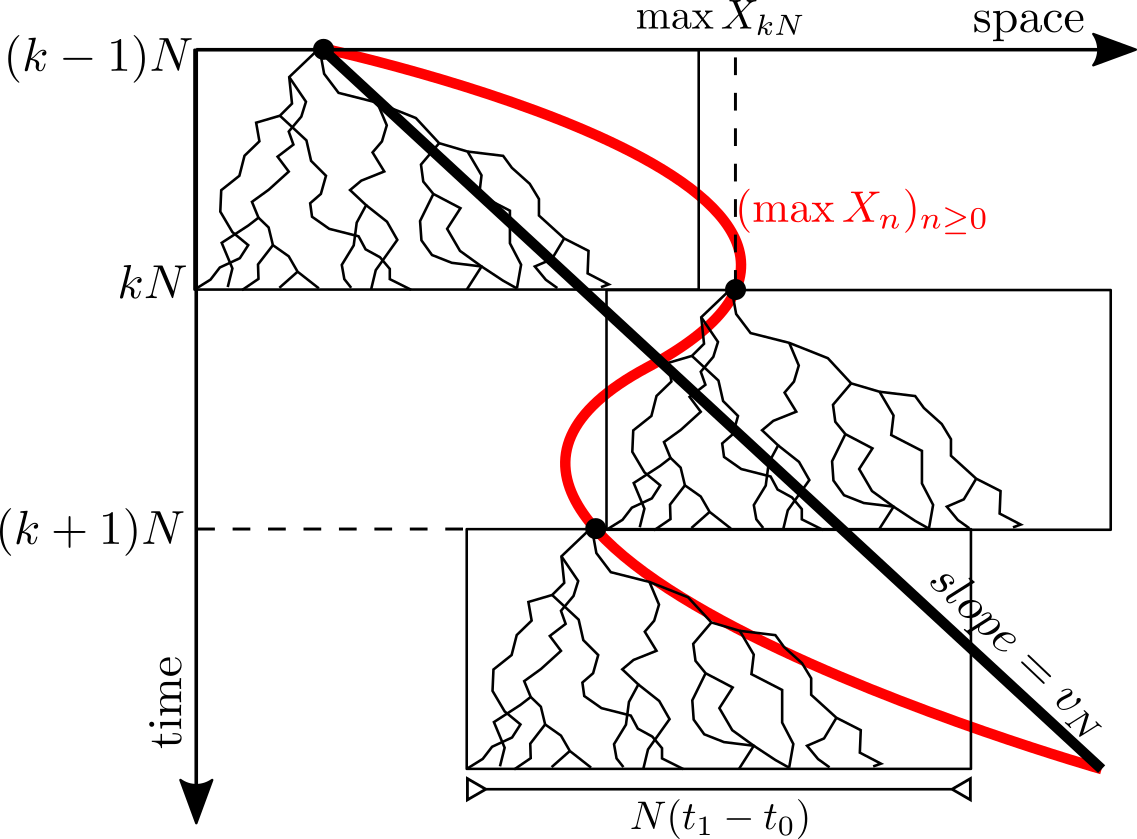
\includegraphics{graphics/g1}
  \caption{Alternative proof of Proposition \ref{prop:diameter}. }
  \label{fig:diam_alternative_proof}
\end{minipage}
\end{figure}

% \begin{wrapfigure}{R}{0.5\textwidth}
% \centering
% 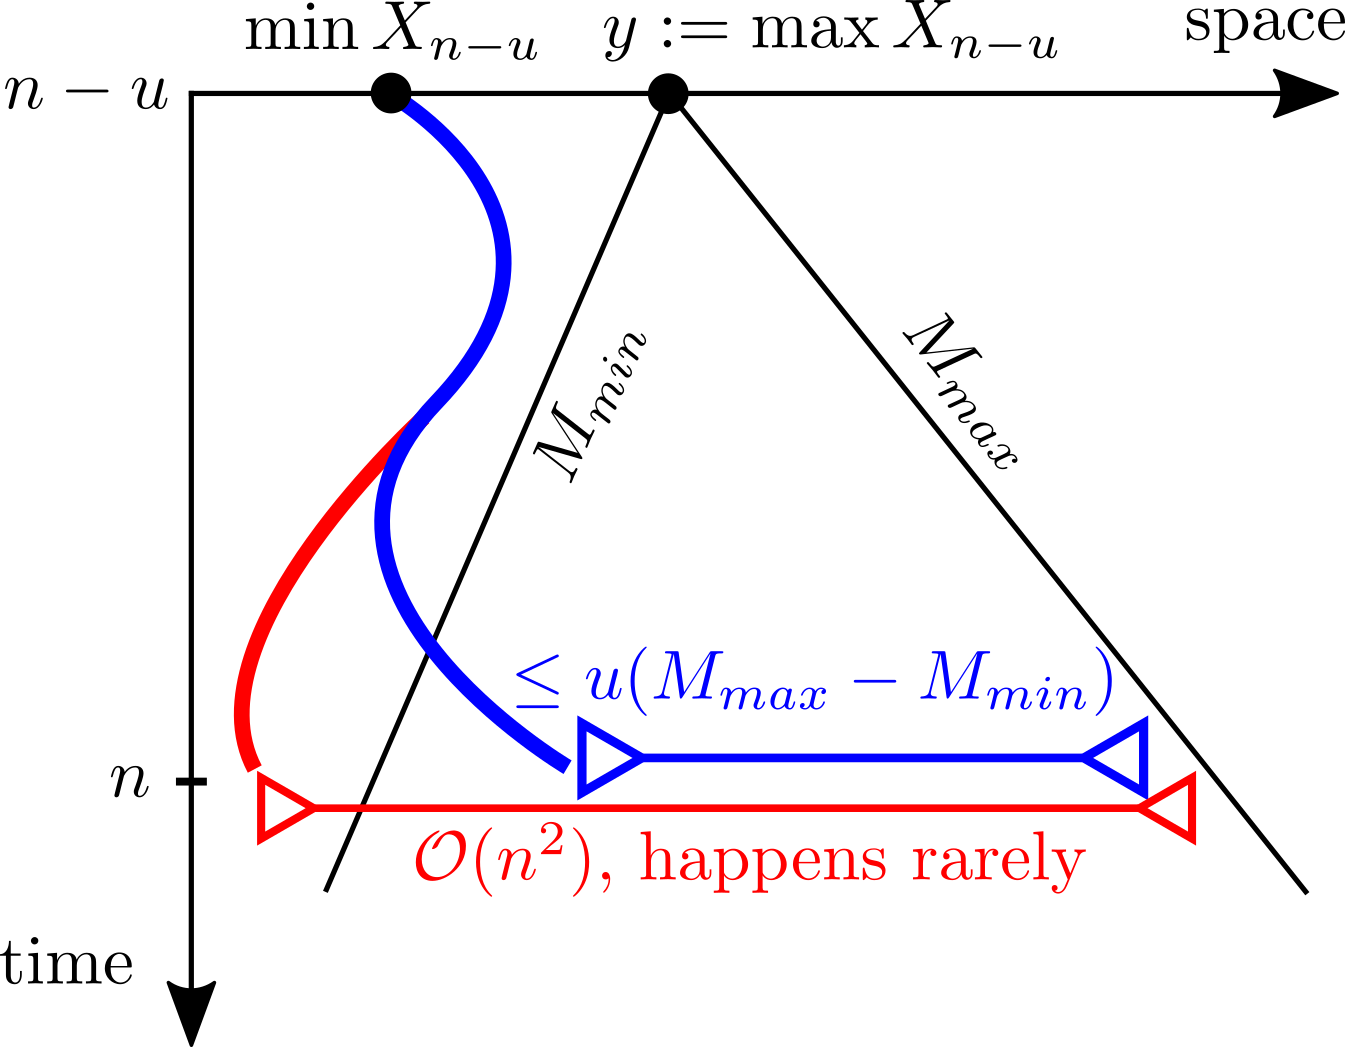
\includegraphics[width=0.45\textwidth]{graphics/g2.png}
% % \caption{\label{fig:frog1}This is a figure caption.}
% \end{wrapfigure}

\begin{proof}[Proof of Proposition \ref{prop:diameter}]
Let $u \in \N_+$ and for $n \geq u$ consider the process $X$ in the timeframe $\bbracket{n - u, n}$. Define 
\begin{align*}
M_{min} &\defeq \min\{ \scr{L}_{i, j}(N) \mid\, i \in \bbracket{n-u, n-1},\, j \in [N]\} \\
M_{max} &\defeq \max\{ \scr{L}_{i, j}(1) = \max\scr{L}_{i,j} \mid\, i \in \bbracket{n-u, n-1},\, j \in [N]\}
\end{align*} 
to be the smallest respectively largest random walk steps made between times $n-u$ and $n$. By Lemma \ref{lem:ExpTailsMax} both $M_{min}$ and $M_{max}$ are integrable. Write $y \defeq \max X_{n - u}$ for the rightmost particle's position at time $n-u$. \\

Suppose that for each $k \in [u]$ we have $\min X_{n - u + k} < y + k m$. As all steps during branching are $ \geq M_{min}$, this implies in particular that the descendants of the particle at space-time point $(y, n-u)$ survive all selection steps until time $n$. Consider a Galton-Watson process $G \defeq (G_n)_{n \geq 0}$ with offspring distribution $\scr{L}$ coupled with the descendants of $(y, n-u)$ and consider the event $A_u \defeq \{ G_u > N\}$. Since $\Ex{\#\scr{L}} > 1$ and $\#\scr{L} \geq 1$ almost surely, $\Pr{A_u} \to 1$ as $u \uparrow \infty$ where $\Pr{A_u}$ is independent of $n$. Since at most $N$ descendants of $y$ can be alive at any time, on $A_u$ we must have $\min X_{n - u + k} \geq y + k_0 M_{min}$ for some $k_0$. By the definition of $M_{min}$ this must also hold for all $k \in \bbracket{k_0, u}$, in particular for $k = u$. Noting that $\max X_n \leq y + u M_{max}$, it follows that 
\begin{equation}\label{eqn:ExpTailDiamUpperBound}
d(X_n)\Ind_{A_u} \leq u (M_{max} - M_{min}), 
\end{equation}
with probability one. Fix $\epsilon > 0$ and take $u$ large enough so that $\Pr{A_u^c} < \epsilon^2$ and consider the decomposition
\begin{equation}\label{eqn:ExpTailsDiamDecomp}
\frac{d(X_n)}{n} = \frac{d(X_n)}{n} \Ind_{A_u} + \frac{d(X_n)}{n} \Ind_{A_u^c}. 
\end{equation}
The reader is referred to Figure \ref{fig:diam_proof} to help understanding. Taking expectations and then taking $n$ to infinity, the first term vanishes by (\ref{eqn:ExpTailDiamUpperBound}). The second term is upper bounded by $(\Pr{A_u^c} \Ex{d(X_n)^2 / n^2})^{1/2}$ using Hölder's inequality. A rough bound on $d(X_n)$ suffices: $d(X_n)$ is stochastically dominated by the sum of $n$ i.i.d. copies of $\max_{j \in [N]} \scr{L}_{0, j}(1) - \min_{j \in [N]} \scr{L}_{0,j}(N)$. Since the $\scr{L}_{n,j}(k)$ have exponentially decaying tails, by Lemma \ref{lem:ExpTailsMax} this yields $\Ex{d(X_n)^2} = \cal{O}(n^2)$ which implies that the second term in \ref{eqn:ExpTailsDiamDecomp} is $\cal{O}(\epsilon)$. Taking $\epsilon$ to zero concludes the proof of $L^1$ convergence. Almost sure convergence is a consequence of the proof of the next Proposition. 
\end{proof}

The original proof of Bérard and Gouéré is identical to ours up to the point where we consider the Galton Watson process $G$. Since they only considered binary BRWs, for $u > \log_2 N$ it is clear that $\Pr{A_u} = 1$ so that there is no need to decompose, they just conclude $d(X_n) \leq u(M_{max} - M_{min}$ almost surely. 

\begin{proposition}[{{\cite[Proposition 2]{exp_tails}}}]\label{prop:ExpTailsSpeedExistence}
There exists $v_N \in \R$ such that for any initial population $X_0 \in \frak{M}_N$ the following holds almost surely and in $L^1$:
\begin{equation}\nonumber
\lim\limits_{n \to \infty} \frac{\min X_n}{n} = \lim\limits_{n \to \infty} \frac{\max X_n}{n} = v_N. 
\end{equation}
\end{proposition}

\begin{proof}
First we treat the case $X_0 = N \delta_0$. Recall the definition of $(\scr{L}_{n, j})_{n \geq 0, j \in [N]}$ from the construction of $X$. For each $l \geq 0$ we define the process $(X^r_n)_{n \geq 0}$ by shifting the origin of time by $r$. More precisely, $X^r_0 = N \delta_0$ for each $r \geq 0$ and given the process up to time $n \geq 0$, $X^r_{n+1}$ is be given by the $N$ rightmost particles of 
\begin{equation}\nonumber
\sum_{j = 1}^N \sum_{l \in \scr{L}_{r + n + 1, j}} \delta_{X^r_n(j) + l}. 
\end{equation}
It is clear that given their initial state, $((X^r_n)_{n \geq 0})_{r \geq 0}$ are identically distributed. In particular, $(X^0_n)_{n \geq 0} = (X_n)_{n \geq 0}$ almost surely. From Lemma \ref{lem:monotonicity} it follows easily that 
\begin{equation}\label{eqn:subadd}
\max X^0_{n + m} \leq \max X^0_n + \max X^n_m \qquad \forall\, n,m \geq 0. 
\end{equation}
For clarity define $Z_{i,j} = \max X^i_{j - i}$ for $0 \leq i \leq j$. Then (\ref{eqn:subadd}) reads $Z_{0, j} \leq Z_{0,i} + Z_{i,j}$ for all $0 \leq i \leq j$, which is familiar territory for Kingman's Subadditive Ergodic Theorem. We postpone showing that the conditions of the theorem hold to Lemma \ref{lem:ExpTailsKingmanHolds}. Applying Kingman's Subadditive Theorem yields 
\begin{equation}\nonumber
\lim_{n \to \infty} n^{-1} \max X_n = \lim_{n \to \infty} \Ex{n^{-1} \max X_n} = \inf_n \Ex{n^{-1} \max X_n} = v_N \in \R
\end{equation}
where the first limit is almost sure. Noting that the process $(-X_n)_{n \geq 0}$ also satisfies the hypothesis of the theorem by our assumptions, we can deduce from the identity $\min X_n = - \max (-X_n)$ that 
\begin{equation}\nonumber
\lim_{n \to \infty} n^{-1} \min X_n = \lim_{n \to \infty} \Ex{n^{-1} \min X_n} = \inf_n \Ex{n^{-1} \min X_n} = \tilde{v}_N \in \R
\end{equation}
exists too, where the first limit is almost sure. From the proof of Proposition \ref{prop:diameter} we immediately get $\tilde{v}_N = v_N$ by uniqueness of $L^1$ limits, which gives $\lim_{n\to\infty} n^{-1}d(X_n) = v_N - \tilde{v}_N = 0$ almost surely as claimed in the previous proposition. The proof is complete in the case $X_0 = N \delta_0$. By translation invariance of the dynamics of the system the result also follows for initial states of the form $N \delta_{x_0}$ for any $x_0 \in \R$. Finally, for arbitrary $X_0 \in \frak{M}_N$ note that the result is a consequence of Lemma \ref{lem:monotonicity} and a sandwiching argument between the initial states $N \delta_{\min X_0}$ and $N \delta_{\max X_0}$. 
\end{proof}

% \begin{wrapfigure}{R}{0.5\textwidth}
% \centering
% 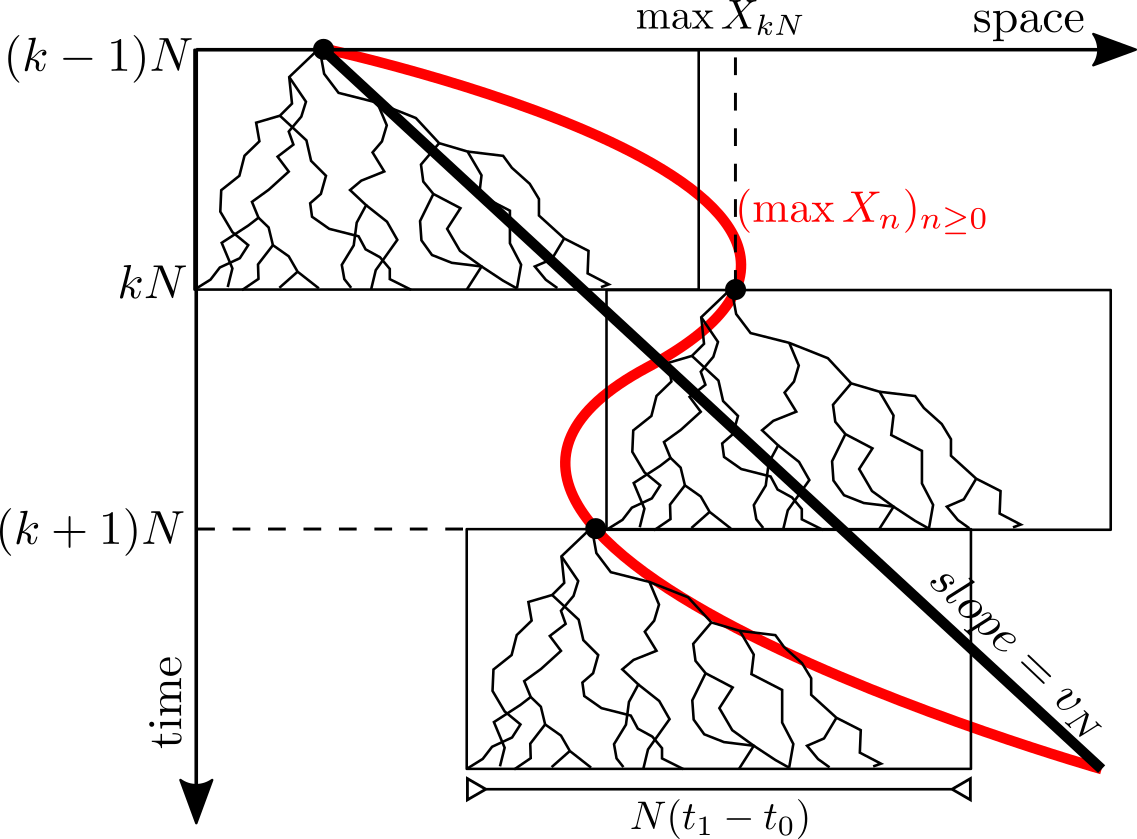
\includegraphics[width=0.45\textwidth]{graphics/g1.png}
% % \caption{\label{fig:frog1}This is a figure caption.}
% \end{wrapfigure}

Inspecting the previous proof, we see that the existence of $v_N$ and $\tilde{v}_N$ (the almost sure and $L^1$ limits of the left- and rightmost particles) when started from $X_0 = N \delta_0$ was shown without relying on Proposition \ref{prop:diameter}. We can in fact deduce Proposition \ref{prop:diameter} by an argument inspired by one of Prof. Berestycki's suggestions:

\begin{proof}[Alternative proof of Proposition \ref{prop:diameter}]
Let $Y = (Y_n)_{n \geq 0}$ be a branching random walk (without selection) with point process $\scr{L}$. Start $Y$ from $\delta_{0}$ noting that initially there is only one particle. Since $\Ex{\# \scr{L}} > 1$ by assumption, the probability $\rho_1$ that the number of particles in $Y$ has reached $N$ by time $N$ is strictly positive. Define $M_{min}$ and $M_{max}$ for $Y$ analogously to their definition in the proof of Proposition \ref{prop:diameter}. By Lemma \ref{lem:ExpTailsMax} one can find $t > 0$ large enough such that $\rho_2 \defeq \PrCond{-t \leq m_Y \leq M_Y \leq t }{\# Y_N \geq N} > 0$. We can now write

\begin{align*}
\Pr{\{ \# Y_N \geq N \} \cap \{-t \leq m_Y \leq M_Y \leq t \}} &= \Pr{\# Y_N \geq N} \PrCond{-t \leq m_Y \leq M_Y \leq t }{\# Y_N \geq N} \\
															   &\geq \rho_1 \rho_2 > 0. 
\end{align*}
Suppose that we couple $X$ with independent copies of $Y$  placed at the space-time points $(\max X_{kN}, kN)_{k \geq 0}$ denoted by $((Y^{(k)}_n)_{0 \leq n \leq N})_{k \geq 0}$. By the second Borel-Cantelli lemma it follows that almost surely infinitely many of the $(Y^{(k)}_n)_{0 \leq n \leq N}$ must have $N$ particles by time $N$ and have $-t \leq m_Y \leq M_Y \leq t $. This in turn implies that for infinitely many $k \geq 0$ the diameter is less than $2Nt$ for some time $n \in [Nk, N(k+1))$. This immediately yields $\tilde{v}_N = v_N$. 
\end{proof}

\begin{proposition}[{{\cite[analogue of Proposition 3]{exp_tails}}}]\label{prop:increasing_speed}
The sequence $(v_N)_{N \geq 1}$ is non-decreasing. 
\end{proposition}
\begin{proof}
This is again a consequence of Lemma \ref{lem:monotonicity}. 
\end{proof}

% \begin{remark}\label{rem:constants}
% From Proposition \ref{prop:increasing_speed} we can deduce that $v_N$ increases to a possibly infinite limit $v_\infty$ as $N$ goes to infinity. Assumption \ref{ass:exponential_tails} implies that $\Lambda$ is smooth on the interior of $\cal{D}(\Lambda)$ so that both quantities $v \defeq \psi'(t^*)$ and $\chi \defeq \frac{\pi^2}{2} t^* \psi''(t^*)$ are finite. In Section \ref{sec:ExpTails_BrunDer} we will see that $v_\infty$ is in fact equal to $v$. 
% \end{remark}





\subsection{Brunet-Derrida behaviour}\label{sec:ExpTails_BrunDer}
First let us describe the coupling between the $N$-branching random walk and $N$ independent branching random walks which allows us apply Theorems \ref{thm:infty_good} and \ref{thm:finite_good}. Let $(\text{BRW}_j)_{j \in [N]} = ((\bb{T}_j, V_j))_{j \in [N]}$ be $N$ independent copies of the BRW with point process $\scr{L}$. Define $\scr{T}_n \defeq \bigsqcup_{j=1}^N \{ x \in \bb{T}_j \,:\, |x|=n \}$ to be the disjoint union of vertices at depth $n$. We now inductively define a sequence $(G_n)_{n \geq 0}$ of random subsets of $\scr{T}_n$, each with exactly $N$ elements. These random subsets will correspond to the particles alive in the coupled $N$-braching random walk at time $n$. Define $G_0 = \scr{T}_0$ and given $G_n$, define $H_n$ to be the vertices in $\scr{T}_{n+1}$ that descend from vertices in $G_n$. Finally, set $G_{n+1}$ to be the set of $N$ vertices in $H_n$ with the gratest value. If we now define (with some abuse of notation) $\frak{X}_n = \sum_{u,j : u \in G_n \cap \bb{T}_j} \delta_{V_j(u)}$ then $(\frak{X}_n)_{n \geq 0}$ has the same distribution as $X$ started from $N \delta_0$. 
% In what follows we will refer to all of $\bb{T}$, $\Phi$, $\epsilon_{n,i,j}$ and $\tau_{n,i}$ without explicitly explaining the obvious relationships between these objects. Let us now record a technical lemma that will be used in the proof of the lower bound in Theorem \ref{thm:ExpTails_BrunDer}. 

\subsubsection{Lower bound}
\begin{proof}[Proof of upper bound in Theorem \ref{thm:ExpTails_BrunDer}]
As before, we first treat the case $X_0 = N \delta_0$. For notational simplicity define $\chi = \pi^2 (t^*)^2 \widehat{\psi}''(t^*) / 2$. Our aim is to show $v_N \defeq \lim_{n \to \infty} \Ex{n^{-1} \max X_n} \leq -  \chi / (\log N)^2 + o((\log N)^{-2})$. Recalling the proof of Proposition \ref{prop:ExpTailsSpeedExistence}, we know by subadditivity that
\begin{equation}\label{eqn:ExpTailsSubaddDecomp1}
v_N \leq \frac{\Ex{\max X_n}}{n} \qquad\qquad\forall\, n \in \N. 
\end{equation}
In light of the desired correction term, we decompose (\ref{eqn:ExpTailsSubaddDecomp1}) into
\begin{equation}\nonumber
\Ex{\max X_n} \leq - \frac{\chi}{(\log N)^2} + \Ex{\max X_n \Ind_{\{\max X_n \geq -n \chi (\log N)^{-2} \}}}. 
\end{equation}
However, this is not the exact form of the RHS that we will work with. Let $\gamma \in (0,1)$ and $\epsilon = \epsilon(N)$ whose precise form we will choose later, but will be approximately $\chi (\log N)^{-2}$ as $N \to \infty$. We go on to show that in
\begin{equation}\nonumber
\Ex{\frac{\max X_n}{n}} \leq  - (1 - \gamma)\epsilon + \Ex{\frac{\max X_n}{n} \Ind_{\{\max X_n \geq  -n (1 - \gamma) \epsilon \}}}
\end{equation}
the last term is $o((\log N)^{-2})$. This will yield the desired upper bound on $v_N$ if we take $\gamma \to 0$. We further decompose the problem: for $\delta > 0$ we have
\begin{equation}\nonumber 
\Ex{\frac{\max X_n}{n} \Ind_{\{\max X_n \geq - n (1 - \gamma)\epsilon \}}} \leq \delta\underbrace{\Pr{\frac{\max X_n}{n} \geq -(1 - \gamma)\epsilon }}_{\circled{1}} + \underbrace{\Ex{\frac{\max X_n}{n} \Ind_{\{ \delta n \leq \max X_n \}}}}_{\circled{2}}. 
\end{equation}
First we show that for an appropriate scaling of $\epsilon=\epsilon(N)$ and $n = n(N)$ we have $\circled{1} = o((\log N)^{-2})$. Set $n = \ceil{N^\xi}$ for some $0 < \xi < \gamma$ and $m = m(N) \leq n$ whose exact form we'll specify soon. Let $B$ be the number of vertices in $\sqcup_{i=0}^n G_i$ that are $(m, - \epsilon)$-good with respect to their corresponding BRWs. Let $u_0, u_1, ..., u_n$ be a path in $\bb{T}_{i_0}$ for some $i_0 \in [N]$ such that $u_0 = root_{i_0}$ and $u_n \in G_n$ with $V_{i_0}(u_n) = \max X_n$. In other words, let $BRW_{i_0}$ be the random walk that the rightmost particle of the coupled $N$-branching random walk lives in at time $n$, and let $u_0, ..., u_n$ be the path connecting it to the corresponding root. Define the event $E \defeq \{ \max X_n \geq - n (1 - \gamma)\epsilon \}$, and apply Lemma \ref{lem:ExpTailsGoodSequencesTechnical} to the sequence of real numbers $(V_{i_0}(u_i))_{i \in [n]}$. It follows that on $E$, for any $K > 0$, either one of the random walk steps along the path is $> K$ or $B \geq \frac{\gamma\epsilon}{K + \epsilon}\frac{n}{m} - \frac{K}{K + \epsilon}$. This yields
\begin{equation}\label{eqn:ExpTailsEBound}
\circled{1} = \Pr{E} \leq \Pr{M \geq K} + \Pr{B \geq \frac{\gamma\epsilon}{K + \epsilon}\frac{n}{m} - \frac{K}{K + \epsilon}},  
\end{equation}
where $M \defeq \max \{\max \scr{L}_{l, j} \mid\, l \in \bbracket{0, n - 1},\, j \in [N]\}$. Set $\beta \in (0, \bb{V}(X))$ and let $\theta > 0$ be as in Theorem \ref{thm:finite_good}. Let $\lambda > 0$, and define 
\begin{equation}\nonumber
m \defeq \ceil*{ \left[\frac{2 \theta}{\pi^2}\right]^{3/2} \left( \frac{(1 + \lambda) \log N}{(\bb{V}(X) - \beta)^{1/2}}\right)^3},
\end{equation} 
and $\epsilon \defeq \theta\, m^{-2/3}$. $m$ is carefully chosen so that by Theorem \ref{thm:finite_good}, 
\begin{equation}\label{eqn:ExpTailsProof}
\rho(m, \epsilon) \leq N^{-(1 + \lambda)} 
\end{equation}
for all large $N$. Also let $K = \kappa \log N$ for $\kappa > 0$ and observe that $\frac{\gamma\epsilon}{K + \epsilon}\frac{n}{m} - \frac{K}{K + \epsilon} > 0$ for large enough $N$ independently of $\kappa$. Thus (\ref{eqn:ExpTailsEBound}) turns into
\begin{equation}\nonumber
\circled{1} = \Pr{E} \leq \underbrace{\Pr{M \geq K}}_{\circled{1a}} + \underbrace{\Pr{B \geq 1}}_{\circled{1b}}. 
\end{equation}

$\circled{1a}$: As noted before, $(\max \scr{L}_{i,j})_{i \geq 0, j \in [N]} = (\scr{L}_{i, j}(1))_{i \geq 0, j \in [N]}$ are i.i.d. with common distribution $\max \scr{L}$ and have exponentially decaying tails so that there exists $C, \phi, K_0 > 0$ such that for all $K > K_0$ it holds that $\Pr{\max \scr{L} > K} \leq C \exp(-\phi K)$. By a calculation similar to the proof of Lemma \ref{lem:ExpTailsMax}, for all large enough $\kappa$ we get
\begin{align}
\Pr{M \geq K} &= 1 - (1 - \Pr{\max \scr{L} > K})^{Nn} \leq 1 - (1 - C \exp(-\phi K))^{Nn} \\
			  &= 1 - (1 - C N^{-\phi \kappa})^{Nn} \leq C N^{-\phi \kappa} Nn = C N^{1 + \xi - \phi \kappa}. 	
\end{align} 
Thus, $\Pr{M \geq K} = o((\log N)^{-2})$ for $\kappa > 2/\phi$. \\

$\circled{1b}$: Consider a vertex $u \in \bb{T}_{j_0}$ for some $j_0 \in [N]$ with $|u| \leq n$. The event $\{u \in G_d\}$ is measurable with respect to the sigma algebra generated by the random variables $\{ V_j(v) \mid\, j \in [N],\, v \in \bb{T}_j,\, |v| \leq |u|\}$. On the other hand, the event $\{ u \text{ is }(m, - \epsilon) \text{-good}\}$ is determined by the variables $\{ V_{j_0}(v) - V_{j_0}(u) \mid\, v \in \bb{T}_{j_0},\, |u| < |v| \}$, so that the two events are independent. We can write $B$ as 
\begin{equation}\nonumber
B = \sum\limits_{i=1}^N \sum\limits_{u \in \bb{T}_i} \Ind_{\{u \text{ is } (m, - \epsilon)\text{-good}\}} \Ind_{\{u \in G_d \text{ for some d} \leq n \}}. 
\end{equation}
Taking expectations gives 
\begin{equation}\nonumber
\Ex{B} \leq N(n+1)\rho(m, \epsilon) = \cal{O}(N^{\xi -\lambda}) = o((\log N)^{-2}) \qquad\text{as $N$ goes to infinity}, 
\end{equation}
where we used that $G_n$ has $N$ elements for all $n$. Applying Markov's inequality to $B$ and combining with our estimate of $\circled{1a}$ gives $\circled{1} = o((\log N)^{-2})$ as desired. \\

We now turn to showing $\circled{2} = o((\log N)^{-2})$. Consider the obvious inequality $\exp(\max X_n) \leq \sum_{j \in [N]} \sum_{x \in \bb{T}_j : |x| = n} \exp(V_j(x))$. It follows from the Many-to-One lemma that 
\begin{align*}
\Ex{\exp(\max X_n)} \leq N\, \E\sum\limits_{|x| = n} \exp(V(x)) = N. 
\end{align*}
Now apply Lemma \ref{lem:ExpTailBound} with $x = \max X_n$ and $a = \delta n$ and take expectations to get 
\begin{align*}
\Ex{\max X_n \Ind_{\{\max X_n \geq \delta n \}}} &\leq \Ex{\exp(X_n - \delta n / 2)} \leq N \, e^{-\delta n / 2} = o((\log N)^{-2}).
\end{align*}
This concludes the proof of the upper bound: we have shown that for any choice of $\gamma \in (0,1)$, $\beta \in (0, \bb{V}(X))$ and $\lambda > \xi > 0$ we have
\begin{equation}\label{eqn:ExpTailResultTally}
v_N \leq \Ex{\ceil{N^\xi}^{-1} \max X_{\ceil{N^\xi}}} \leq - (1 - \gamma) \frac{\pi^2 (\bb{V}(X) - \beta)}{2 (1 + \lambda)^2(\log N)^2} + o((\log N)^{-2}). 
\end{equation}
Taking $\gamma, \beta, \lambda$ and $\xi$ to zero gives the desired result. 
\end{proof}

Here is a summary of the variables used in the previous proof, collected in a table to ease understanding
\begin{center}
\begin{tabular}{|c|c||c|c|} 
 \hline
 % Variable 	& Definition 			& Variable 	& Definition 								            \\
 $\gamma$ 	& $\in (0, 1)$ 			&	$\bb{V}(X)$		& $2 \chi / \pi^2$		        \\

 $\delta$ 	& $\in (0, \infty)$ 	&  	$\beta$			& $\in (0, \bb{V}(X))$								            \\ 

 $\xi$ 		& $\in (0, \gamma)$ 	&	$\theta$	& as in Theorem \ref{thm:finite_good}			                             \\ 

 $\kappa$	& $\in (0, \infty)$		&	$K$ 				& $\kappa \log N$	                 \\

$\chi$ 			& $\pi^2 (t^*)^2 \widehat{\psi}''(t^*) / 2$ &  $m$ & $\ceil*{ \left[\frac{2 \theta}{\pi^2}\right]^{3/2} \left( \frac{(1 + \lambda) \log N}{(\bb{V}(X) - \beta)^{1/2}}\right)^3}$\\

$\lambda$	& $\in (0, \infty)$ & $\epsilon$ & $\theta\,m^{-2/3}$ \\

$n$ 		& $\ceil{N^\xi}$     & & \\

 \hline
\end{tabular}
\end{center}










\subsubsection{Upper bound}
\begin{proof}[Proof of lower bound in Theorem \ref{thm:ExpTails_BrunDer}]

Let $\lambda, \eta \in (0,1)$ and let 
\begin{equation}\nonumber
\epsilon \defeq \frac{\chi}{(1-\lambda)^2(\log N)^2}. 
\end{equation}
With this choice Theorem \ref{thm:infty_good} gives $\rho(\infty, - \epsilon) = N^{\lambda - 1 + o(1)}$ as $N \to \infty$. Recall now the construction of $(X^r_n)_{n, l \geq 0}$ using $(\scr{L}_{n, j})_{n \geq 0, j \in [N]}$ from the proof of Proposition \ref{prop:ExpTailsSpeedExistence}. Define the random variables $\Gamma_0 \defeq 0$ and $J_0 \defeq 0$ and set $i = 0$. Given $\Gamma_i$ and $J_i$ inductively define $L_{i+1} \defeq n \land \inf\{ k \mid\, \min X^{\Gamma_i}_k \geq -(1+\eta)\epsilon k\}$. Finally, let $\Gamma_{i+1} \defeq \Gamma_i + L_{i+1}$ and $J_{i+1} \defeq J_i + \min X^{\Gamma_i}_{L_{i+1}}$. By Lemma \ref{lem:monotonicity} it follows that 
\begin{equation}\label{eqn:regenTime}
\min X_{\Gamma_i} \geq J_i \qquad\forall\, i \geq 0. 
\end{equation}
Observe now that $\Gamma_{i+1} - \Gamma_i$ is an i.i.d. sequence with common distribution $L \defeq n \land \inf \{ k \mid \min X_k \geq - (1+\eta)\epsilon k\}$. Similarly, the sequence $J_{i+1} - J_i$ is also i.i.d. with common distribution $\min X_L$. The strong law of large numbers gives 
\begin{equation}
\lim\limits_{i \to \infty} \frac{\min X_{\Gamma_i}}{i} = \lim\limits_{i \to \infty} \frac{\min X_{\Gamma_i}}{\Gamma_i} \frac{\Gamma_i}{i} = v_N \E L
\end{equation}
almost surely. However, by (\ref{eqn:regenTime}) we also have
\begin{equation}
\liminf\limits_{i \to \infty} \frac{\min X_{\Gamma_i}}{i} \geq \liminf\limits_{i \to \infty} \frac{J_i}{i} = \Ex{\min X_L}.
\end{equation}
Denote $B \defeq \{ \min X_k < - (1+\eta)\epsilon \text{ for all } k \in [n]\}$ and define the random variable $\Theta_n$ to have the law of $\min \{\min \scr{L}_{i, j} \mid\, j \in [N],\, 0 \leq i \leq n - 1 \}$. Combining the obvious inequalities $\min X_L \geq -(1 + \eta)\epsilon L \Ind_{B^c} + n \Theta_n \Ind_B$ and $1 \leq L \leq n$ with the above bounds we get
\begin{equation}\label{eqn:lowerBdd}
v_N \geq \frac{\Ex{\min X_L}}{\E L} \geq -(1+\eta)\epsilon (1 + n\Pr{B}) - n\Ex{|\Theta_n| \Ind_B}. 
\end{equation}
By Hölder's inequality $\Ex{|\Theta_n| \Ind_B} \leq \sqrt{\Ex{\Theta_n^2}\Pr{B}}$. By Lemma \ref{lem:ExpTailsMax} we know that $\Theta_n$ has exponentially decaying tails, so in particular is square-integrable. To prove the lower bound we only need a suitably strong upper bound on $\Pr{B}$. The remainder of the proof is dedicated to this. \\

Since $1 < \Ex{\#\scr{L}} = \E\sum_{|x|=1} \Ind$, by the monotone convergence theorem we can take $R \in \R$ such that $1 < \E\sum_{|x|=1} \Ind_{\{ V(x) \geq R\}}$. If we let $(M_n)_{n \geq 0}$ be the Galton Watson process started from $M_0 = 1$ with offspring law $\sum_{|x|=1} \Ind_{\{ V(x) \geq -R\}}$ then by Lemma \ref{lem:ExpTailsGW} there exist $\phi > 1$ and $r > 0$ such that $\Pr{M_n \geq \phi^n} \geq r$ for all $n \geq 0$. Define now $s \defeq \ceil{\frac{\log N}{\log \phi}} + 1$ and $m \defeq \ceil{\frac{- Rs}{\eta\, \epsilon}}$ and finally set $n = s + m$. Consider a vertex $u$ at depth $m$ in one of the $BRW_i$. The probability that there are at least $\phi^s$ distinct paths $u \eqdef u_m, ..., u_n$ with $V_i(u_{k+1}) - V_i(u_k) \geq R$ for all $k \in \bbracket{m, n - 1}$ is greater than $r$ by our previous discussion. Recall that the probability of the root being $(m, - \epsilon)$-good is $\rho(m, - \epsilon)$. We see that then the probability of observing a path $root = w_0, ..., w_n$ in $BRW_i$ such that $V_i(w_k) \geq - k \epsilon$ for $k \in [m]$ and $V_i(w_{k+1}) - V_i(w_k) \geq R$ for $k \in \bbracket{m, n-1}$ is at least $\rho(m, - \epsilon) r$. By the choice of $s$ and $m$, such a path must also be $(n,  - (1+\eta)\epsilon)$-good. For $i \in [N]$ define $A_j$ to be the event that $BRW_i$ contains no more than $\phi^s$ distinct $(n, - (1+\eta)\epsilon)$-good paths starting at the root. By independence we get
\begin{equation}
\Pr{\bigcap\limits_{i=1}^N A_i} \leq (1 - \rho(m, \epsilon) r)^N. 
\end{equation}
On the event $B \cap [\cap_{i=1}^N A_i]^c$ one of the $BRW_i$s has $> \phi^s > N$ particles at time $n$ that have stayed to the right of the space time line with slope $ - (1 + \eta)\epsilon$ until time $n$. By definition, on $B$ this implies that there are $> N$ particles alive in the $N$-branching random walk which is impossible. Therefore we must have $B \subset \cap_{i=1}^N A_i$. Using the fact that $\rho(m, - \epsilon) \leq \rho(\infty, - \epsilon) = N^{\lambda - 1 + o(1)}$ and the inequality $1 - x \leq \exp(-x)$ for all $x \in \R$, we get
\begin{equation}\label{eqn:ExpTailsBBound}
\Pr{B} \leq \Pr{\bigcap\limits_{i=1}^N A_i} \leq \exp(-N^{\lambda + o(1)})
\end{equation}
Combining the above estimate of $\Pr{B}$ with (\ref{eqn:lowerBdd}) results in 
\begin{equation}
v_N \geq - \frac{\chi (1 + \eta)}{(1 - \lambda)^2(\log N)^2} + o((\log N)^{-2}). 
\end{equation} 
As $\lambda$ and $\eta$ can be taken arbitrarily small, the desired result follows. 
\end{proof}

\subsection{Discussion}
This section is based in part on \cite{exp_tails} Section 8. Write $v_N$ for the asymptotic speed of the $N$-BRW and $v \defeq \lim_{N \to \infty} v$ for its limit, to which it converges at rate $(\log N)^{-2}$. The proof of the Brunet-Deridda behaviour hinged on the idea that the following two are comparable:
\begin{enumerate}[(a)]
\item \vspace{-1mm} $(BRW_j)_{j \in [N]}$ do not survive killing below the speed $v - \epsilon$
\item \vspace{-3mm} $v_N < v - \epsilon$. 
\end{enumerate}
\vspace{-3mm}
It is intuitively clear why this might be true: if $(a)$ holds then we certainly can't expect the $N$-BRW to propagate faster than $v - \epsilon$ since it is dominated by $(BRW_j)_{j \in [N]}$ through the coupling introduced in section \ref{sec:ExpTails_BrunDer}. Conversely, suppose $(a)$ doesn't hold. Consider the particle in the $N$-BRW at time zero that corresponds to a $BRW_i$ that survives killing. With probability $ \sim 1/N$ the descendants of this particle will survive and form the entirety of the $N$-BRW. If this doesn't happen we can `restart' the argument. After a rougly geometric number of attempts we will succed in which case $(b)$ cannot hold. \\

To make such an argument rigorous we needed to get a handle on the probability of a $BRW$ exhibiting paths of various slopes and lengths near the critical slope $0$; the expectation of the $BRW$'s associated random walk. In \cite{gantert2008asymptotics} they did just that using the Many-to-One lemma and one of Mogulskii's results which accurately describes the probabilitiy of a centred random walk's path to stay in a general space-time region. Loosely speaking they show that on the scale $m \propto \epsilon^{-u}$ for $u \in (0, 3/2]$ we have
\begin{equation}
\log \rho(m, -\epsilon) \propto - \epsilon^{-u/3}\qquad\text{as } \epsilon \downarrow 0. 
\end{equation}
Similarly, they show $\log\rho(\infty, -\epsilon) \propto - \epsilon^{1/2}$ as $\epsilon \downarrow 0$. Using this the convergence rate $(\log N)^{-2}$ can be heuristically deduced: setting $\epsilon_N = v - v_N$ we would expect 
\begin{equation}\label{eqn:speed_scale_heuristic}
\rho(\infty, - \epsilon_N) \propto \frac{1}{N}. 
\end{equation}
To see why, suppose for contradiction that $\rho(\infty, - \epsilon_N) \ll 1_N$. Then with probability close to one none of the $BRW_i$ survive killing which would imply that $v_N$ needs to be slower. Conversely, if we had $\rho(\infty, - \epsilon_N) \gg 1/N$ then with probability close to one at least one of the $BRW_i$ would survive killing, implying that $v_N$ needs to be faster. From \ref{eqn:speed_scale_heuristic} and the asymptotic form of $\rho(\infty, -\epsilon)$ for small $\epsilon$ it follows that for all large $N$, $\epsilon_N$ should satisfy
\begin{equation}
\epsilon_N \propto (\log N)^{-2}. 
\end{equation}

\subsection{$\alpha$-stable spine}

In \cite[Lemma 4.2]{mallein2018n} Mallein studies a generalisation of the model we considered in this section. Recall that if $(\bb{T}, V)$ is a $BRW$ with point process $\scr{L}$ that satisfies (\ref{eqn:BRW_V_Ass}) i.e.
\begin{equation}
e^{\psi(1)} = \E \sum\limits_{|x|=1} e^{V(x)} = 1, 
\end{equation}
then the step distribution of the spine $X$ is given by
\begin{equation}
\Pr{X \leq x} = \E \sum\limits_{|u| = 1} \Ind_{\{V(u) \leq x\}} e^{V(u)}. 
\end{equation}
In Section \ref{sec:light_tails} we considered the case when $X$ had finite mean and variance so that by the central limit theorem it belonged to the domain of attraction of the Gaussian law. Mallein puts less stringent conditions on $X$: he requires that $X$ be in the domain of attraction of some stable random variable $Y$ that veryfies $\Pr{Y \geq 0} \in (0, 1)$. The family of stable probability distributions are often referred to as $\alpha$-stable distributions, signifying the dependence on the parameter $\alpha \in (0, 2]$. The case $\alpha = 2$ corresponds to the Gaussian while for $\alpha \in (0, 2)$ we get $\alpha$-regularly varying distributions (for a definition see Section \ref{sec:poly}). He defines the truncated second moment function
\begin{equation}
L^*(x) \defeq x^{\alpha - 2} \Ex{Y^2 \Ind_{|Y| \leq x}}, 
\end{equation}
and goes on to show that under some further technical conditions on $\scr{L}$ that we omit, it holds that 
\begin{equation}
v_N \sim - C_* \frac{L^*(\log N)}{(\log N)^\alpha} \qquad\text{as } N \to \infty
\end{equation}
for $C_* > 0$ depending on $Y$ whose form he also specifies. 

\newpage
\section{POLYNOMIAL TAILS}\label{sec:poly}

\begin{quote}
{\small Placeholder text. }
\end{quote}

\subsection{Overview of heavy tailed distributions}\label{sec:heavy_tailed_overview}
In this section we rely on sections 2 and 3 of \cite{foss2011introduction}. For a random variable $X$ with cumulative distribution function $F$, let $\overline{F}(x) \defeq \Pr{X > x} = 1 - F(x)$ be its right tail-function. $F$ is said to be heavy-tailed if 
\begin{equation}\label{eqn:heavy_tailed_distr_def}
\int_\R e^{\lambda x} dF = \infty\qquad\forall\, \lambda > 0. 
\end{equation}
$F$ is said to be light-tailed if it is not heavy-tailed. It is clear that if $F$ is positive and light-tailed then it has finite moments of all orders. A positive function $f : \R \to \R_+$ is said to be heavy-tailed if 
\begin{equation}\label{eqn:heavy_tailed_fn_def}
\limsup\limits_{x \to \infty} e^{\lambda x} f(x) = \infty\qquad\forall\,\lambda > 0. 
\end{equation}
We have the following characterisation of heavy tailed distributions:

\begin{theorem}[{{\cite[Theorem 2.6, adapted]{foss2011introduction}}}]
Let $F$ be a distribution function. The following are equivalent:
\begin{itemize}
\item $F$ is heavy-tailed in the sense (\ref{eqn:heavy_tailed_distr_def})
\item $\overline{F}$ is heavy-tailed in the sense (\ref{eqn:heavy_tailed_fn_def}). 
\end{itemize}
If any of the above holds and $F$ has density $f$ with respect to the Lebesgue measure, then $f$ is also heavy-tailed. The converse however is not true in general. 
\end{theorem}

Let $f$ be a positive function as before. For a positive, non-decreasing function $h:\R \to \R_+$ we say that $f$ is $h$-insensitive if 
\begin{equation}\label{eqn:h_insensitive_def}
\lim\limits_{x \to \infty} \sup\limits_{|y| \leq h(x)} \left\lvert \frac{f(x+y)}{f(x)} - 1 \right\rvert = 0. 
\end{equation}
If $f$ is $h$-insensitive for all constant functions $h$ we say that $f$ is long-tailed. For $f$ to be long-tailed, $h$-insensitivity for some $h$ with $h(\infty) = \infty$ is obviously sufficient (and also necessary by Lemma 2.19 \cite{foss2011introduction}). Furthermore $f$ being long-tailed implies that $f$ is heavy-tailed by Lemma 2.17 \cite{foss2011introduction}. By varying the choice of $h$, we can classify long-tailed functions according to the heaviness of their tails. An important subset of long-tailed functions are those of regular variation: A positive function $f:\R \to \R_+$ is said to be regularly varying at $\infty$ with index $\alpha \in \R$ if for all $c > 0$, 
\begin{equation}
f(cx) \sim c^\alpha f(x) \qquad\text{ as } x \to \infty. 
\end{equation}
Functions that are $0$-regularly varying are called slowly varying. It is a well known result that if $f$ is $\alpha$-regularly varying then it can be written as $f(x) = x^\alpha f_0(x)$ for some slowly varying $f_0$. The definitions of long-tailedness and regular variation naturally extend to probability distributions $F$: we say $F$ is regularly varying with index $\alpha > 0$ if $\overline{F}$ is regularly varying with index $- \alpha$. A probability distribution having long-tails has a simple probabilistic interpretation: the distribution function $F$ is long-tailed by definition if 
\begin{equation}\label{eqn:long_tail_interpretation}
\PrCond{X > x + y}{X > x} \to 1 \qquad\text{ as } x \to \infty\,, \forall\, y > 0, 
\end{equation}
where $X$ has distribution $F$. Notice that this doesn't give uniform convergence in $y$ on closed intervals as required by definition (\ref{eqn:h_insensitive_def}), however it is a standard result that the two are equivalent. Interpreting (\ref{eqn:long_tail_interpretation}) in words, given that $F$ exceeds some high level the probability of it exceeding an even higher level is large. Finally, we introduce the class of subexponential functions: a distribution $F$ is called subexponential if it is long-tailed and 
\begin{equation}\label{eqn:subexponential_def}
\overline{F * F} (x) \sim 2 \overline{F}(x) \qquad\text{ as } x \to \infty, 
\end{equation}
where $*$ denotes convolution. (\ref{eqn:subexponential_def}) in fact implies $\overline{F^{* (n)}} \sim n \overline{F}$ for $n \geq 1$ so that we have the following probabilistic interpretation: if $(X_i)_{1 \leq i \leq n}$ is an i.i.d. sequence with common distribution $F$ then 
\begin{equation}
\Pr{X_1 + ... + X_n > x} \sim \Pr{\max\limits_{1 \leq i \leq n} X_i > x} \qquad\text{ as } x \to \infty. 
\end{equation}
Let $\cal{H}, \cal{L}, \cal{S}, \cal{R}$ denote the class of heavy-tailed, long-tailed, subexponential and regularly varying probability distributions respectively. We have the following inclusions:
\begin{equation}
\cal{R} \subset \cal{S} \subset \cal{L} \subset \cal{H}, 
\end{equation}
where the leftmost inclusion is a consequence of Theorem 3.29 \cite{foss2011introduction}. Probability distributions arising in practice virtually always fall in the class of light-tailed distributions or that of the subexponential distributions.  



% Potter's bounds (\cite[Section 6]{poly_tails}) provide a powerful tool for working with regularly varying functions. The result says that for any $C > 1$ and $\delta > 0$ there exist $R \in \R$ such that 
% \begin{equation}
% \frac{f(y)}{f(x)} \leq C \left( \frac{y}{x} \right)^{\alpha + \delta} \lor \left( \frac{y}{x} \right)^{\alpha -\delta} \qquad\forall\, x,y \geq R. 
% \end{equation}





\subsection{The result}\label{sec:poly_result}
Here we present the model as studied in \cite{poly_tails}. Let $(X_n)_{n \geq 0}$ be the $N$-BRW evolving as follows: At each step each particle gives birth to two children whose position is distributed independently and identically around the position of the parent, according to the law of a random variable $X$. Then, out of all children the $N$ rightmost are selected tp form the next generation where $N \geq 2$ is fixed. The authors further impose the condition $X \geq 0$ almost surely and that the random variable $X$ be regularly varying with index $\alpha > 0$. The authors remark that the methods of their analysis could be extended to more general reproduction laws and to $X$ taking values in $\R$, however since no new phenomena can be observed the don't do so. For $x \geq 0$ define $h$ to be given by
\begin{equation}
\Pr{X > x} \eqdef \overline{F}(x) \eqdef \frac{1}{h(x)}. 
\end{equation} 
Then our assumptions imply that $h$ is regularly varying at infinity with index $\alpha$. Define the sequence $(c_N)_{N \geq 1}$ by $c_N \defeq h^{-1} (2N \log_2 N)$ where $h^{-1}(x) \defeq \inf\{ y :\, h(y) > x\}$ is the generalised inverse of $h$. Let $\cal{L}(Y)$ denote the law of the random variable $Y$ and let $d(\cdot, \cdot)$ be the Prokhorov metric on the space of probability distributions on $\R$, which induces the topology of weak convergence. We now present Theorem 1.2 of \cite{poly_tails} as it is found there. 

\begin{theorem}[{{\cite[Theorem 1.2]{poly_tails}}}]\label{thm:poly_tails_result}
We distinguish the following cases:
\begin{enumerate}[(a)]

\item \vspace{-2mm} $\alpha > 1$: The limits $v_N \defeq \lim_{n \to \infty} n^{-1} \max X_n = \lim_{n \to \infty} n^{-1} \min X_n$ exist almost surely and in $L^1$ and satisfies $v_N \sim \rho_\alpha c_N / \log_2 N$ as $N \to \infty$ where $\rho_\alpha > 0$. \\

\item \vspace{-6mm} $\alpha = 1,\, \E X < \infty$: $v_N$ exists as above and satisfies 
\begin{equation}
v_N \sim \frac{c_N h(c_N)}{\log_2 N} \int\limits^\infty_1 \frac{1}{h(x c_N)} dx \qquad\,\text{as }N \to \infty. \\
\end{equation}

\item \vspace{-7mm} $\alpha = 1,\, \E X = \infty$: Let $b_n = \int\limits^{h^{-1}(n)}_{1} h(c_N)/h(c_N x) dx$. For $i=1$ and $i=N$ we have
\begin{equation}\nonumber
\lim\limits_{N \to \infty} \limsup\limits_{n \to \infty} d(\cal{L}\left( \frac{\log_2 N}{c_N}\frac{X_n(i)}{n b_n}\right), \delta_1) = 0. 
\end{equation}

\item \vspace{-5mm} $\alpha \in (0, 1)$: Let $W_\alpha$ be the random variable whose moment generating function is given by
\begin{equation}\nonumber
\E e^{-\lambda W_\alpha} = exp(- \alpha \int\limits^\infty_0 (1 - e^{-\lambda x})x^{-\alpha - 1}dx). 
\end{equation}
Then for $i=1$ and $i=N$, 
\begin{equation}\nonumber
\lim\limits_{N \to \infty} \limsup\limits_{n \to \infty} d(\cal{L}\left( \frac{1}{(2N)^{1/\alpha}}\frac{X_n(i)}{h^{-1}(n)}\right), \cal{L}(W_\alpha)) = 0. 
\end{equation}
\end{enumerate}
\end{theorem}

The way Bérard and Maillard show this is by considering a stochastic process which they call the `stairs process'. As opposed to the light tailed models considered in Section \ref{sec:light_tails}, when the tails are heavy the cloud of particles moves mainly through large occasional jumps. The stairs process is devised so that it mimics this behaviour. They prove certain properties of these stairs processes, most importantly their asymptotic speed of propagation when suitably scaling space and time, which is the subject of Theorem 2.5 \cite{poly_tails}. Using delicate couplings between the $N$-BRW and the continuous and discretized stairs processes, they obtain that $c_N^{-1} \max X_n$ converges to the stairs process in the $J_1$ topology while the minimum converges in the $M_1$. \\

From Theorem \ref{thm:poly_tails_result} it is hard to tell what $v_N$ looks like in practice because of expressions like $c_N$, $h^{-1}(c_N)$. In Section \ref{sec:examples} we present a fully worked example as well as simulations which should give us an idea of what these processes look like. From our discussion in Section \ref{sec:heavy_tailed_overview} we know that Bérard and Maillard didn't cover all classes of heavy-tailed distributions, in particular examining what happens for distributions in $\scr{S} \setminus \scr{L}$ might be the subject of future research.


 % We briefly describe the stairs process to gain some intuition about Bérard and Maillard's argument. \\

% Further define $(\xi_t)_{t \geq 0}$ by $\xi_t = x$ iff $(t, x)$ is an atom of $\cal{P}$ and zero otherwise. 

% Let $\mu_\alpha$ be the measure on $[0, \infty)$ defined by $\mu_\alpha([x, \infty)) = x^{-\alpha}$. Let $\cal{P}$ be a Poisson point process on $\R_+^2$ with intensity $dt \otimes \mu_\alpha$ i.e. let $\cal{P}$ be a random measure on $\R_+^2$ such that for any Borel measurable $G \in \scr{B}(\R_+^2)$ and $n \in \N$ we have $\Pr{\cal{P}(G) = n} = \Pr{\dPo{\int_G dt \otimes \mu_\alpha} = n}$. We will think of the first coordinate as time and of the second as space. The corresponding stairs process $\cal{R}^\alpha \defeq (\cal{R}^\alpha (t))_{t \geq 0}$ is then defined as follows: Suppose that $\cal{R}^\alpha$ is already defined for times $ \leq n$. Now generate the points in the interval $(n, n+1] \times \R_+$ according to $\cal{P}$ and translate every atom $(t,x)$ by $\cal{R}^\alpha (t-1)$ in the space direction. Finally, define $\cal{R}^\alpha$ to be the record process of these points for the time interval $(n, n+1]$. See the introduction of \cite{poly_tails} for two alternate characterisations of $\cal{R}^\alpha$. Bérard and Maillard obtain the following result relating the stairs process and the $N$-BRW with $\alpha$-regularly varying tails:

% \begin{theorem}[{{\cite[Theorem 1.1]{poly_tails}}}]
% With notation as above, 
% \begin{align*}
% (c_N^{-1} \max X(\floor{t \log_2 N)})_{t \geq 0} &\rightarrow (\cal{R}^\alpha (t))_{t \geq 0} \qquad&&\text{ in } J_1, \\ 	
% (c_N^{-1} \max X(\floor{t \log_2 N}), c_N^{-1} \min X(\floor{t \log_2 N}))_{t \geq 0} &\rightarrow (\cal{R}^\alpha (t), \cal{R}^\alpha (t - 1))_{t \geq 0} \qquad&&\text{ in } M_1. 
% \end{align*}
% \end{theorem}

\newpage
\section{EXAMPLES}\label{sec:examples}
As before, let $(X_n)_{n \geq 0}$ be the $N$-BRW governed by the point process $\scr{L}$ with logarithmic moment generating function $\psi$. In this section we provide some concrete examples and reflect upon how they fit into the previous sections' results. 







\subsection{Binary Gaussian N-BRW}\label{subsec:examples_gaussian_BRW}
Suppose that $\scr{L} = \delta_{Y_1} + \delta_{Y_2}$ where $Y_1, Y_2$ are i.i.d. normal with mean $\mu$ and variance $\sigma^2 > 0$. The logarithmic moment generating function takes the form
\begin{equation}\nonumber
\psi(t) = \log \Ex{e^{Y_1} + e^{Y_2}} = \mu t + \frac{\sigma^2 t^2}{2} + \log 2. 
\end{equation}
Clearly $\psi(t)$ is finite for all $t \in \R$, and solving for $t^* > 0$ in $\psi'(t^*) t^* = \psi(t^*)$ we get $t^* = \sqrt{\frac{2 \log 2}{\sigma^2}}$. Therefore $\scr{L}$ satisfies the hypothesis of Theorem \ref{thm:ExpTails_BrunDer_non_transformed}, and so 
\begin{equation}\nonumber
\lim\limits_{n \to \infty} \frac{\max X_n}{n} = v_N = \mu + \sqrt{\sigma^2 \log 4} - \frac{\pi^2 \sqrt{\sigma^2 \log 4}}{2 (\log N)^2} + o((\log N)^{-2}). 
\end{equation}
In fact, we could replace the Gaussian distribution with any distribution on $\R$ that has finite moment generating function on all of $\R$ and which puts less than $1/2$ mass on its essential supremum. The resulting point process would still satisfy the hypothesis of Theorem \ref{thm:ExpTails_BrunDer_non_transformed} by Proposition \ref{prop:jaffuel}. \\





\begin{figure}[!h]
\centering
\begin{minipage}{0.45\textwidth}
  \centering
  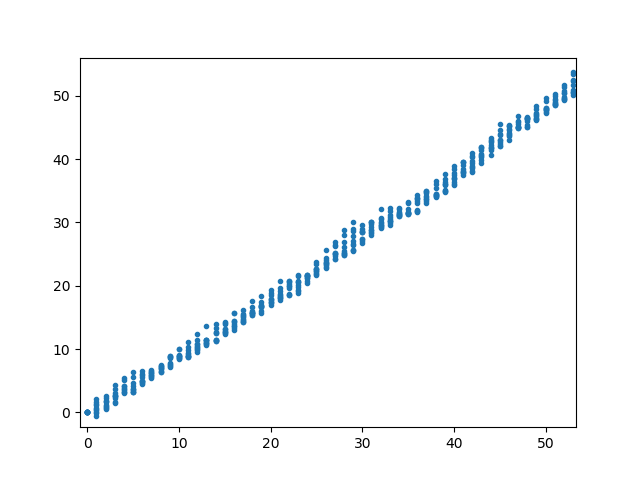
\includegraphics[width=.99\linewidth]{graphics/std_normal}
  \caption{Gaussian binary $N$-BRW with $N = 10$}
  \label{fig:normal}
\end{minipage}\hfill
\begin{minipage}{0.45\textwidth}
  \centering
  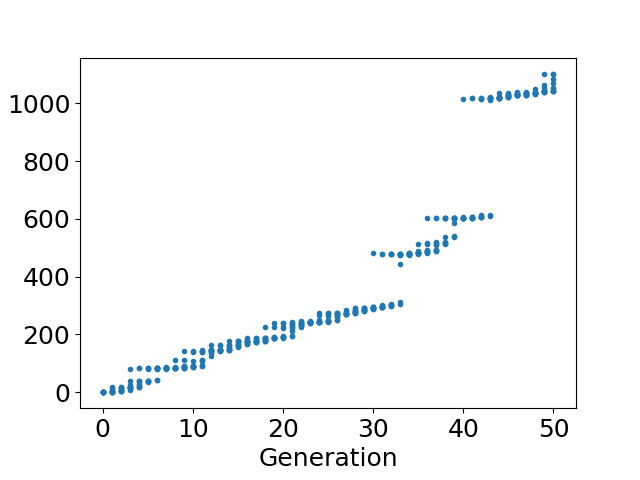
\includegraphics[width=.99\linewidth]{graphics/cauchy}
  \caption{Cauchy binary $N$-BRW with $N = 10$. }
  \label{fig:cauchy}
\end{minipage}\hfill%
\end{figure}






\subsection{Binary Bernoulli N-BRW}\label{subsec:binary_bernoulli_BRW}
Another natural choice might be $Y_1, Y_2$ i.i.d. Bernoulli with parameter $\alpha \in (0, 1)$. However, it turns out that the hypothesis of Theorem \ref{thm:ExpTails_BrunDer_non_transformed} is satisfied if and only if $\alpha \in (0, 1/2)$. This is because for $\alpha \geq 1/2$ the $Y_i$ put $\geq 1/2$ mass on their essential supremum (which in this case is equal to $1$). \\

To see this consider the following. $\psi(t) = \log 2 + \log (\alpha e^t + 1 - \alpha)$ so if $f(t) \defeq t \psi'(t) - \psi(t)$ then $f'(t) = t \psi''(t) > 0$ for all $t > 0$. Now, as $f(0) = -\log 2 < 0$, the equation $f(t^*) = 0$ has a solution $t^* > 0$ if and only if $\lim_{t \to \infty} f(t) > 0$. We have
\begin{align*}
\lim\limits_{t \to \infty} f(t) &= \lim\limits_{t \to \infty} \left[\frac{\alpha t e^t}{\alpha e^t + 1 - \alpha} - \log(\alpha e^t + 1 - \alpha) - \log 2 \right] \\
								&= \lim\limits_{t \to \infty} \left[ t \big( 1 - \frac{1 - \alpha}{\alpha e^t + 1 - \alpha}\big) - t - \log (1 + \frac{1-\alpha}{\alpha} e^{-t}) - \log(2 \alpha) \right] \\
								&= - \log(2\alpha). 
\end{align*} 
Above expression is positive if and only if $\alpha \in (0, 1/2)$ as claimed. In \cite{exp_tails} Bérard and Gouéré note this as well and go on to show the following
\begin{theorem}[{{\cite[Theorems 4, 5]{exp_tails}}}]
For $\alpha = 1/2$ it holds that
\begin{equation}\nonumber
1 - v_N = \Theta(N^{-1})
\end{equation}
while for $\alpha \in (1/2, 1]$ we have
\begin{equation}\nonumber
- \log (1 - v_N) = \Theta(N). 
\end{equation}
\end{theorem}
\begin{remark}A slightly more general case of Bernoulli $N$-BRWs was studied by the authors \cite{couronne2014branching} using elementary methods, making it an accessible and enjoyable read. 
\end{remark}


\begin{figure}[!h]
\centering
\begin{minipage}{0.45\textwidth}
  \centering
  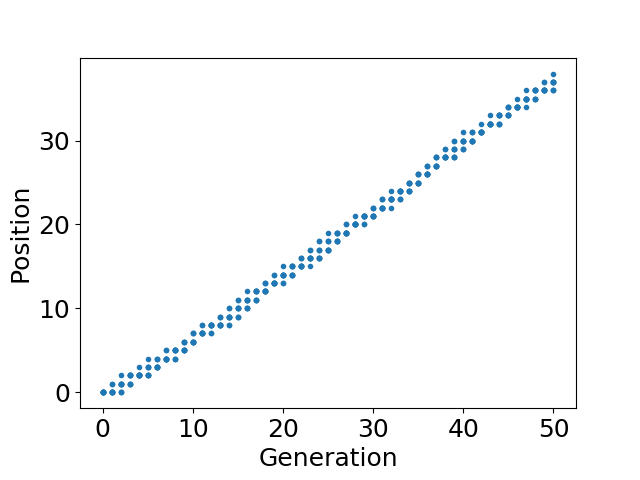
\includegraphics[width=.99\linewidth]{graphics/bernoulli_25}
  \caption{Bernoulli binary $N$-BRW with $N=10, p=0.25$. }
  \label{fig:ber25}
\end{minipage}\hfill
\begin{minipage}{0.45\textwidth}
  \centering
  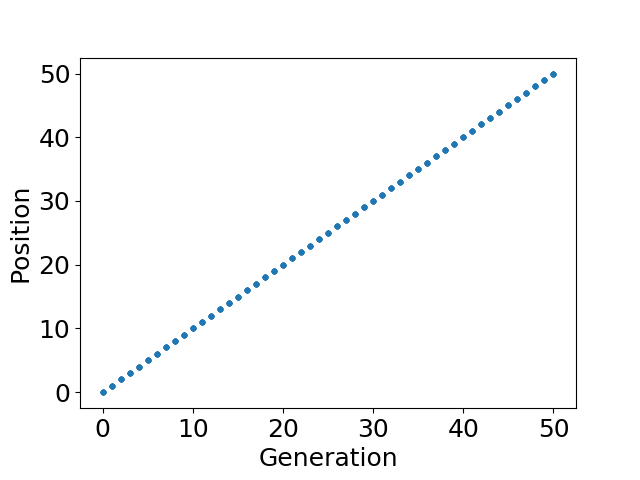
\includegraphics[width=.99\linewidth]{graphics/bernoulli_75}
  \caption{Bernoulli binary $N$-BRW with $N=10, p=0.75$. }
  \label{fig:ber75}
\end{minipage}\hfill%
\end{figure}




% \subsection{N-BBM}
% % Let $(B_t)_{t \geq 0}$ be a standard Branching Brownian Motion (as described in Section \ref{sec:examplessubsec:FKPP}) that branches at rate $\beta$ each time giving birth to $M$ particles. Standard BBM corresponds to the case $\beta = 1$ and $M = 2$. 
% Let $(B_t)_{t \geq 0}$ be a standard $N$-BBM (as described in Section \ref{subsec:FKPP}) started from $N\,\delta_0$. Clearly $(B_n)_{n \in \N}$ is an $N$-BRW, however explicitly describing its point process is not trivial. Nevertheless, its logarithmic moment generating function is easy to obtain. It is clear that $\# \scr{L}$ is distributed as the simple birth process $(M_t)_{t \geq 0}$ after one unit of time that is started from $M_0 = 1$ with escape rate equal to the number of particles alive. It is an elementary fact that $\E M_t = e^t$ so we get
% \begin{equation}\nonumber
% \psi(t) = 1 + \frac{t^2}{2}. 
% \end{equation}
% Solving $\psi'(t^*) t^* = \psi(t^*)$ we obtain $t^* = \sqrt{2}$. By Theorem \ref{thm:ExpTails_BrunDer_non_transformed} we get
% \begin{equation}\nonumber
% v_N \defeq \lim\limits_{n \to \infty} \frac{\max B_n}{n} = \sqrt{2} - \frac{\pi^2}{\sqrt{2}(\log N)^2} + o((\log N)^{-2})
% \end{equation}
% where the limit is both in $L^1$ and almost surely. We can use a simple sandwiching argument to get the corresponding result for continuous time. We have
% \begin{equation}\label{eqn:sandwich}
% \frac{\max B_t}{t} = \bigg( \frac{\max B_t - \max B_{\floor{t}}}{\floor{t}} + \underbrace{\frac{\max B_{\floor{t}}}{\floor{t}}}_{\to v_N\,a.s.\,\&\,L^1} \bigg) \underbrace{\frac{\floor{t}}{t}}_{\to 1}. 
% \end{equation}
% Fix $t \geq 0$ and let $\cal{P} \defeq (P_j)_{j \in [N]}$ be an i.i.d. collection of $\dPo{1}$ random variables. Further, let $\cal{Z} \defeq (Z^{j, k}_t)_{j \in \N,\,k \geq 1,\, t \geq 0}$ be a collection of i.i.d. standard Brownian motions independent of $\cal{N}$. There is an obvious coupling of $(B_s)_{\floor{t} \leq s < t}$ and the collections $\cal{P}$ and $\cal{Z}$. This coupling immediately yields the following upper bound: 
% \begin{equation}
% \max B_t - \max B_{\floor{t}} \stackrel{st.}{\leq} \sum\limits_{j=1}^N \sum\limits_{k=1}^{P_j} \sup\limits_{s \in [0, 1)} Z^{j, k}_s. 
% \end{equation}
% It is a well known fact that $\sup_{s \in [0, 1)} Z_s$ and $|Z_1| \in L^1$ have the same distribution for a standard Brownian motion $(Z_t)_{t \geq 0}$. In the same fashion we can obtain a lower bound and we find that
% \begin{equation}
% |\max B_t - \max B_{\floor{t}}| \stackrel{st.}{\leq} \cal{B}
% \end{equation}
% where the distribution of $\cal{B} \in L^1$ is independent of $t$. This gives $t^{-1} \max B_t \to v_N$ in $L^1$ while almost sure convergence follows by the Borel-Cantelli lemma. Indeed, let $(\cal{B}_j)_{j \geq 0}$ be an i.i.d. collection distributed like $\cal{B}$. Then
% \begin{equation}\nonumber
% \Pr{t^{-1} \max B_t \nrightarrow v_N} \leq \sum\limits_{k = 1}^\infty \Pr{\cal{B}_n > n/k \text{ for infinitely many }n \in \N} = 0, 
% \end{equation}
% since $\int_0^\infty \Pr{\cal{B} > \lambda} d\lambda = \E\cal{B} < \infty$. 


% Clearly by the Markov property, for any $t \geq 0$ we have
% \begin{equation}
%  \max B_t - \max B_{\floor{t}} \leq \sup\limits_{s \in [0, 1)} \left[ \max B_{\floor{t} + s} - \max B_{\floor{t}} \right] \stackrel{st.}{\leq} \sup\limits_{s \in [0, 1)} \max B_s. 
% \end{equation}

% This


% \begin{equation}\nonumber
% \scr{L} = \sum\limits^P_{j=1} \delta_{Y_j}, 
% \end{equation}
% where $P \sim 1 + \dPo{\beta}$ and $Y_j \sim \dNorn{0, 1}$ for $j = 1, 2, ...$ are all independent. By a simple calculation
% \begin{equation}\nonumber
% \psi(t) = \log
% \end{equation}


\subsection{N-BRW with Cauchy spine}
Consider the model where $\scr{L}$ is given by a Poisson Point Process with intensity measure $e^{-x} \nu_\alpha (dx)$ where $\nu_\alpha$ is some $\alpha$-stable distribution with $\nu_\alpha(0, \infty) \in (0, 1)$. By The Slivnyak-Mecke Theorem \cite[Theorem 1.13]{baccelli2009stochastic} we have
\begin{equation}\nonumber
\E \sum\limits_{l \in \scr{L}} e^l = \int_\R e^\lambda e^{-\lambda} \nu_\alpha(d\lambda) = 1
\end{equation}
so $\scr{L}$ satisfies (\ref{eqn:BRW_V_Ass}). We claim that the spine is in the domain of attraction of $\nu_\alpha$. Indeed, we just have to observe that 
\begin{equation}
\Pr{X \leq x} \defeq \E \sum\limits_{l \in \scr{L}} \Ind_{\{ l \leq x \}} e^l  = \int\limits^x_{-\infty} \nu_\alpha(d \lambda), 
\end{equation}
 by the Slivnyak-Mecke theorem. Since stable distributions are in their own domains of attraction (\cite[p. 576]{feller1957introduction}) we are done. 

\begin{remark}
In Figure \ref{fig:Cauchy_spine} we see a simulation of the above model. Producing the image was not entirely straightforward: the PPP with intensity $p_\alpha (dx) = e^{-x} \nu_\alpha (dx)$ has almost surely infinitely many points on the negative real line. Thus we cannot generate the entirety of the Cauchy PPP - it is enough to generate the rightmost $N$ points. To do so we had to make use of multiple properties of PPPs: if $A, B \subset \R$ are disjoint then the number and position of points in $A, B$ are independent. Furthermore the number of points in $A$ is a Poisson random variable with mean $\int_A p_\alpha(dx)$ conditional on which the position of points is i.i.d. with unnormalised density $p_\alpha$ on $A$. To make simulations reasonably fast we also had to make use of the fact that PPPs are additive and that $e^{-x}/(1+x^2)$ can be integrated in closed form.  
\end{remark}

\begin{figure}[!h]
  \centering
  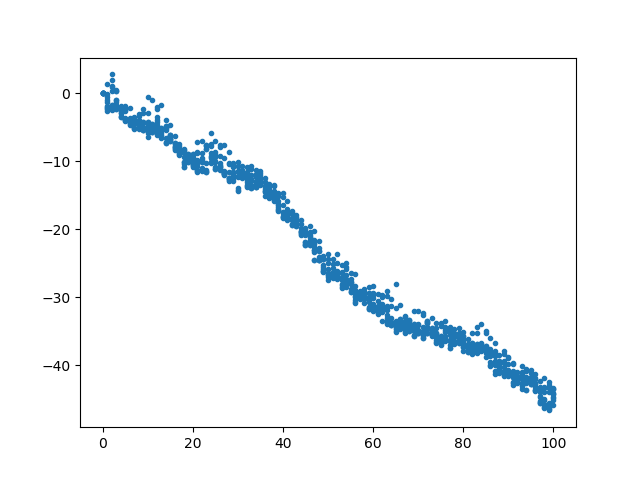
\includegraphics[width=.99\linewidth]{graphics/cauchy_PPP}
  \caption{$N$-BRW with Cauchy spine. }
  \label{fig:Cauchy_spine}
\end{figure}


\subsection{Binary N-BRW with polynomial tails}
As in Sections \ref{subsec:examples_gaussian_BRW} and \ref{subsec:binary_bernoulli_BRW}, let $\scr{L} = \delta_{Y_1} + \delta_{Y_2}$ where this time $Y_1, Y_2$ are i.i.d. with distribution given by
\begin{equation}
\Pr{Y_1 > x} = \frac{1}{x^\alpha},\qquad\forall\,x \geq 1
\end{equation}
for some $\alpha > 0$. If $\alpha > 1$ we can use the notation of Section \ref{sec:poly_result} to get $c_N = (2N \log_2 N)^{1/\alpha}$ so that
\begin{equation}\nonumber
v_N \sim \frac{\rho_\alpha c_N}{\log_2 N} \propto \left( \frac{N}{(\log N)^{\alpha - 1 }} \right)^{1/\alpha}
\end{equation}
by Theorem \ref{thm:poly_tails_result}. For $\alpha = 1$ we are in case $(c)$ of Theorem \ref{thm:poly_tails_result} and we have $c_N = 2 N \log_2 N$ and $b_N = \int^n_1 dx/x = \log n + \cal{O}(1)$. Thus loosely speaking we get 
\begin{equation}
\frac{\max X_n}{n \log n} \approx \delta_{2N}. 
\end{equation}
It is worth noting that in both of these cases the behaviour of the system is vastly different from the Brunet-Derrida behaviour. In particular, the speed at which the particles propagate diverges as $N \to \infty$. 
\newpage

\section{Appendix}\label{sec:appendix}
\begin{lemma}\label{lem:ExpTailsMax}
Let $\tau \in L^1$ be an $\N$-valued random variable and let $(\epsilon_n)_{n \geq 1}$ be an i.i.d. sequence of random variables with exponentially decaying tails, independent of $\tau$. Then $M \defeq \max_{1 \leq n \leq \tau} \epsilon_n$ has exponentially decaying tails. 
\end{lemma}

\begin{proof}
Let $C, \gamma, t_0 > 0$ be such that $\Pr{|\epsilon_1| \leq t} \geq 1 - C e^{- \gamma t}$ for all $t > t_0$. Then for $t > t_0$ large enough, Bernoulli's inequality gives 
\begin{align*}
\Pr{M > t} &\leq 1 - \Ex{\Pr{|\epsilon_1| \leq t}^\tau} \leq 1 - \Ex{(1 - C e^{-\gamma t})^\tau} \\
		   &\leq 1 - \Ex{1 - C e^{- \gamma t} \tau} = \underbrace{C\, \Ex{\tau}}_{< \infty} e^{- \gamma t}. 
\intertext{Similarly, looking at the lower tail we get}
\Pr{M < -t} &\leq 1 - \Ex{\Pr{|\epsilon_1| \leq t}^\tau} \leq C\, \Ex{\tau} e^{- \gamma t}. 
\end{align*}
\end{proof}

\begin{lemma} \label{lem:ExpTailBound}
For all large enough $a$, 
\begin{equation}
x \Ind_{\{x \geq a\}} \leq e^{x - a/2}, \qquad\forall\, x \in \R. 
\end{equation}
\end{lemma}
\begin{proof}
Differentiate the map $f:x \mapsto \exp(x - a/2) - x$ to find that for large enough $a$, f is increasing on $[a, \infty)$. Noting that $f(a) \geq 0$ for all large $a$ concludes the proof.  
\end{proof}

\begin{lemma}\label{lem:ExpTailsGW}
Let $(M_n)_{n \geq 0}$ be a supercritical Galton-Watson process with offspring distribution $X$ and let $\mu \defeq \E X > 1$. If $M_0 = 1$ then for all $\mu > \phi > 0$ we have $0 < \liminf_n \Pr{M_n > \phi^n}$. 
\end{lemma}

\begin{proof}
By the monotone convergence theorem we can take $R$ large enough so that $\widetilde{\mu} \defeq \Ex{R \land X} > 1$. Let $(\widetilde{M}_n)_{n \geq 0}$ be the Galton-Watson process with offspring distribution $\widetilde{X} \defeq R \land X$ which by assumption is also supercritical. As $\widetilde{X}$ is bounded, Theorem 1 in Section 6, Chapter 1 of \cite{athreya2004branching} gives $\widetilde{\mu}^{-n} \widetilde{M}_n \to M$ almost surely for some $M \geq 0$ with $\Pr{M > 0} > 0$ by Theorem 2 of the same section. By the obvious coupling 
\begin{equation}
\Pr{M_n > \phi^n} \geq \Pr{\widetilde{M}_n \mu^{-n} > \phi^n \mu^{-n}}
\end{equation} 
so that $\liminf_{n \to \infty} \Pr{M_n > \phi^n} \geq \Pr{M > 0} > 0$. 
\end{proof}

\begin{theorem}[{{\cite[Theorem 7.4.1.]{durrett2010probability}}}]
Let $\{X_{m,n} \mid\, 0 \leq m < n\}$ be a family of random variables satisfying 
\begin{enumerate}[(i)]
\item $X_{0,n} \leq X_{0,m} + X_{m, n}$ for all $m < n$. 
\item $(X_{nk, (n+1)k})_{n \geq 0}$ is a stationary and ergodic sequence for each $k \geq 1$. 
\item The distribution of $\{X_{m + k, n + k} \mid\, 0 \leq m < n\}$ does not depend on $k \in \N$. 
\item $\Ex{X_{0,1}^+} < \infty$ and there exists $\gamma_0 > -\infty$ such that $\Ex{X_{0,n}} > \gamma_0 n$ for all $n \in \N$. 
\end{enumerate}
Then there exists $\gamma \in \R$ such that 
\begin{equation}
\lim\limits_{n \to \infty} \frac{\E X_{0, n}}{n} = \inf\limits_{n} \frac{\E X_{0,n}}{n} = \gamma, 
\end{equation}
where the last limit is almost sure and in $L^1$. 
\end{theorem}

\begin{lemma}\label{lem:ExpTailsKingmanHolds}
The random variables $Z_{i,j}$ as defined in the proof of Proposition \ref{prop:ExpTailsSpeedExistence} satisfy the hypothesis of Kingman's Subadditive Theorem. 
\end{lemma}

\begin{proof}
For each $k \geq 1$ the sequence $\{Z_{k, 2k}, Z_{2k, 3k}, ...\} = \{\max X^k_k, \max X^{2k}_k, ... \}$ is i.i.d. so stationary and ergodic. Clearly the distribution of $(Z_{i, i + k})_{k \geq 0} = (\max X^i_k)_{k \geq 0}$ is independent of $i$. $\E Z^+_{0,1} = \E (\max X_1)^+ < \infty$ because $\max X_1 \in L^1$ by (\ref{eqn:ExpTailsMaxIntegrable}). Finally, $\E Z_{0, n} = \E \max X_n \geq n\, \E \scr{L}_{0,1}(1)$. 
\end{proof}

\begin{lemma}[{{\cite[Adapted by Bérard and Gouéré from Lemma 5.2]{pemantle2009search}}}]\label{lem:ExpTailsGoodSequencesTechnical}
Let $v_1 < v_2 \in \R$ and $1 \leq m \leq n \in \N$. Suppose $0 \eqdef x_0, ..., x_n$ is a sequence of real numbers such that $\max_{i \in \bbracket{0, n - 1}} (x_{i+1} - x_i) \leq K$ for some $K > 0$, and define $I \defeq \{ i \in \bbracket{0, n - m} \mid\, x_{i + j} - x_i \geq j v_1,\quad \forall j\in\bbracket{0,m}\}$. If $x_n \geq v_2 n$, then $\#I \geq \frac{v_2 - v_1}{K - v_1}\frac{n}{m} - \frac{K}{K - v_1}$. 
\end{lemma}

\newpage

\section{CODE FOR SIMULATIONS}

\subsection{Figures \ref{fig:normal}, \ref{fig:cauchy}, \ref{fig:ber25} and \ref{fig:ber75}}
\inputminted[obeytabs=true,tabsize=2]{python}{simulations/simulation(for_show).py}

\subsection{Figure \ref{fig:Cauchy_spine}}
\inputminted[obeytabs=true,tabsize=2]{python}{simulations/PPP_simulation(for_show).py}
\newpage

\bibliographystyle{plain}
\bibliography{bibliography}

\end{document}
